% =============================================================================
% Post-Quantum Cryptography Migration Survey
% Target: IEEE Communications Surveys & Tutorials
% Template: IEEEtran (journal mode)
% Authors: [To be filled]
% Date: July 2026
% =============================================================================

\documentclass[journal]{IEEEtran}

% ----------------------------- Packages --------------------------------------
\usepackage{cite}
\usepackage{amsmath,amssymb,amsfonts}
\usepackage{algorithmic}
\usepackage{algorithm}
\usepackage{graphicx}
\usepackage{textcomp}
\usepackage{xcolor}
\usepackage{booktabs}
\usepackage{multirow}
\usepackage{array}
\usepackage{tabularx}
\usepackage{longtable}
\usepackage{rotating}
\usepackage{hyperref}
\usepackage{url}
\usepackage{microtype}
\usepackage{enumitem}
\usepackage{tikz}
\usepackage{pgfplots}
\pgfplotsset{compat=1.18}
\usepackage{pgf-pie}
\usepackage{subcaption}
\usepackage{float}
\usepackage{listings}
\usepackage{mdframed}
\usepackage{cleveref}

% Listings style for pseudocode
\lstset{
  basicstyle=\footnotesize\ttfamily,
  breaklines=true,
  frame=single,
  numbers=left,
  numberstyle=\tiny,
  keywordstyle=\bfseries\color{blue!70!black},
  commentstyle=\itshape\color{green!50!black},
  stringstyle=\color{red!60!black}
}

% Definition box for frameworks
\newmdtheoremenv{definition}{Definition}
\newmdtheoremenv{theorem}{Theorem}

% Custom column types
\newcolumntype{L}[1]{>{\raggedright\arraybackslash}p{#1}}
\newcolumntype{C}[1]{>{\centering\arraybackslash}p{#1}}
\newcolumntype{R}[1]{>{\raggedleft\arraybackslash}p{#1}}

% Hyphenation corrections
\hyphenation{op-tical net-works semi-conduc-tor post-quan-tum crypto-gra-phy}

% =============================================================================
\begin{document}
% =============================================================================

% ----------------------------- Title -----------------------------------------
\title{A Comprehensive Survey on Post-Quantum Cryptography Migration:\\
Standards, Threat Models, Implementation Challenges, and\\
Regulatory Roadmaps for Legacy Systems}

\author{Allan~Douglas~Costa%
\thanks{Manuscript received July 15, 2026.}%
\thanks{A.~D.~Costa is with the Institute of Cyberspace (ICIBE),
Federal Rural University of the Amazon (UFRA), Bel\'{e}m, PA, Brazil.
E-mail: allan.costa@ufra.edu.br.
ORCID: \href{https://orcid.org/0000-0002-7068-8889}{0000-0002-7068-8889}.}%
\thanks{This work was supported by the Amazon Foundation for the
Support of Studies and Research (FAPESPA), the Information and
Communication Technology Company of the State of Par\'{a} (PRODEPA),
and the National Education and Research Network (RNP).}%
}

\markboth{IEEE Communications Surveys \& Tutorials,~Vol.~XX, No.~XX, 2026}%
{A.~D.~Costa: Post-Quantum Cryptography Migration Survey}

\maketitle

% =============================================================================
% ABSTRACT
% =============================================================================
\begin{abstract}
The imminent realization of fault-tolerant quantum computers threatens to render
RSA and elliptic-curve cryptography (ECC), foundational to virtually all
contemporary secure communications, fundamentally insecure. Shor's algorithm
solves the integer factorization and discrete logarithm problems in polynomial
time, eliminating the computational hardness upon which RSA-2048 and ECC-256
rely for security guarantees expected to last decades. The National Institute of
Standards and Technology (NIST) finalized the first post-quantum cryptography
(PQC) standards in August 2024: FIPS~203 (ML-KEM), FIPS~204 (ML-DSA), and
FIPS~205 (SLH-DSA), triggering mandatory migration timelines across critical
sectors worldwide. Despite this pivotal standardization milestone, no
comprehensive survey has systematically mapped the migration landscape across
standards evolution, threat models, domain-specific implementation constraints,
and divergent regulatory frameworks.

This survey addresses that gap by providing a unified taxonomy of PQC
migration challenges spanning six critical infrastructure domains: Transport
Layer Security (TLS), Public Key Infrastructure (PKI), Internet of Things (IoT),
Blockchain and distributed ledger technologies, Virtual Private Networks (VPN)
and Zero Trust architectures, and Industrial Control Systems (ICS/OT). Through
a structured narrative review encompassing 151 peer-reviewed
publications and 39 normative/standards documents (2016--2026, with seminal
antecedents), we identify 14 distinct migration strategies and compare their
applicability across these domains. We introduce the Migration
Readiness Classification (MRC) framework, a heuristic decision-support rubric,
that scores legacy systems across four tiers
(Critical, High, Medium, and Low readiness) based on cryptographic exposure,
upgrade feasibility, and regulatory deadline proximity.

Our structured comparison reveals critical implementation gaps not addressed by
current NIST guidance: performance overhead remains prohibitive for ultra-constrained
devices with fewer than 64~KB of RAM; we identified no evidence in the reviewed
corpus of automated cryptographic inventory tools covering the majority of
enterprise attack surfaces; and regulatory frameworks
across the United States, European Union, and Brazil exhibit substantive alignment
gaps that complicate multinational compliance strategies. Quantum key distribution
(QKD) approaches remain impractical for most enterprise deployments due to cost
and distance limitations based on evidence in the reviewed corpus,
reinforcing the primacy of algorithm-based PQC.
Critically, current crypto-agility assumptions embedded in NIST guidance exhibit
brittleness when applied to constrained device classes typical of industrial
control environments.

This survey provides researchers, practitioners, and policymakers with a
structured roadmap for evidence-based PQC migration decision-making, supported
by reproducible analysis code and a curated dataset.
\end{abstract}

% ----------------------------- Keywords --------------------------------------
\begin{IEEEkeywords}
Post-Quantum Cryptography, Structured Narrative Survey, NIST PQC Standards,
Legacy System Migration, ML-KEM, ML-DSA, SLH-DSA, FN-DSA, Crypto-Agility,
Harvest Now Decrypt Later, Critical Infrastructure Security, Regulatory Compliance,
Migration Readiness Classification, Lattice-Based Cryptography, Hash-Based Signatures
\end{IEEEkeywords}

% =============================================================================
% SECTION I: INTRODUCTION
% =============================================================================
\section{Introduction}
\label{sec:intro}

\IEEEPARstart{T}{he} intersection of quantum computing progress and global digital
infrastructure creates one of the most consequential security challenges of the
coming decade. Contemporary public-key cryptographic systems, including RSA~\cite{rivest1978method},
Diffie-Hellman key exchange~\cite{diffie1976new}, and elliptic-curve variants, derive
their security from the computational intractability of integer factorization and
discrete logarithm problems. Shor's quantum algorithm~\cite{shor1994algorithms}
renders both problems solvable in polynomial time on a sufficiently large
quantum computer, invalidating the security assumptions underlying billions of
deployed cryptographic implementations.

\subsection{The Quantum Computing Threat Landscape}

Quantum computing has transitioned from theoretical construct to engineering
reality. In 2019, Google demonstrated ``quantum supremacy'' on a 53-qubit
Sycamore processor~\cite{arute2019quantum}. By 2023, IBM achieved 1,121
operational qubits on its Condor processor~\cite{ibm2023condor}, and in 2024
demonstrated a 133-qubit Heron chip with substantially reduced error rates.
Google's Willow chip (2024) further reduced below-threshold error rates.
While current noisy intermediate-scale quantum (NISQ) devices cannot yet
execute Shor's algorithm against cryptographic key sizes, the trajectory of
progress suggests cryptographically relevant quantum computers (CRQCs) may
emerge within 10--15 years~\cite{mosca2018cybersecurity,preskill2018quantum}.

The key vulnerability surface is vast. An estimated 4.4 billion SSL/TLS
certificates worldwide rely on RSA or ECC for key exchange~\cite{netcraft2024survey}.
Critical infrastructure sectors (financial systems, healthcare, energy grids,
telecommunications, and government communications) collectively depend on
public-key cryptography for authentication, key establishment, and data
confidentiality. The ``Harvest Now, Decrypt Later'' (HNDL) threat
compounds urgency: adversaries can intercept and store encrypted traffic
today and decrypt it retroactively once CRQCs become available~\cite{chen2016report,
nsasuite2022}. Data with multi-decade confidentiality requirements (classified
government communications, medical records, intellectual property) is thus
already at risk.

\subsection{The Standardization Inflection Point}

NIST's Post-Quantum Cryptography Standardization project, initiated in
2016~\cite{nist2016call}, concluded its primary phase in August 2024 with the
publication of three Federal Information Processing Standards:
\begin{itemize}
  \item \textbf{FIPS~203} (ML-KEM): Module-Lattice-Based Key-Encapsulation
  Mechanism, derived from CRYSTALS-Kyber~\cite{nistfips203};
  \item \textbf{FIPS~204} (ML-DSA): Module-Lattice-Based Digital Signature
  Algorithm, derived from CRYSTALS-Dilithium~\cite{nistfips204};
  \item \textbf{FIPS~205} (SLH-DSA): Stateless Hash-Based Digital Signature
  Algorithm, derived from SPHINCS+~\cite{nistfips205}.
\end{itemize}
FALCON has been standardized as FN-DSA (FIPS~206, August 2024), an NTRU-lattice-based
signature scheme optimized for compact signatures~\cite{nistfips206}.
HQC, a code-based KEM selected for standardization in 2025, will constitute
an algorithmic diversity backup~\cite{aragon2022hqc}.

These standards trigger mandatory migration obligations across federal agencies
(via OMB M-23-02~\cite{omb2023m2302}) and propagate through supply chains
into critical infrastructure sectors, financial regulation, and healthcare.
The NSA's Commercial National Security Algorithm Suite 2.0 (CNSA~2.0)~\cite{nsacnsa2022}
mandates adoption timelines ranging from 2025 (software/firmware) to 2033
(legacy systems). European counterparts from ENISA~\cite{enisa2022pqc} and
national agencies establish parallel but not always aligned requirements.

\subsection{Why a Survey Now?}

The post-2024 standardization environment creates a critical need for synthesis.
Existing surveys address PQC algorithms in isolation~\cite{bernstein2017postquantum,
nejatollahi2019post}, or focus on specific domains such as IoT~\cite{liu2021pqc},
TLS~\cite{stebila2020postquantum}, or blockchain~\cite{fernandezcarames2020review}.
To our knowledge, no single prior survey simultaneously:
\begin{enumerate}
  \item Systematically covers all six critical infrastructure domains under a common framework;
  \item Follows PRISMA~2020 reporting principles (transparent selection criteria,
  documented exclusion rationale, corpus composition diagram) for a
  migration-focused research question, while explicitly acknowledging that
  database search execution against indexed repositories remains a planned
  future step (Section~\ref{sec:methodology});
  \item Introduces a structured migration readiness rubric applicable across sectors;
  \item Maps global regulatory divergence with implementation implications;
  \item Identifies AI/ML acceleration opportunities for migration planning.
\end{enumerate}

Table~\ref{tab:survey_comparison} compares this survey against the six most
relevant prior surveys along these five dimensions.

\begin{table*}[t]
\caption{Comparison of This Survey With Prior PQC Survey Works}
\label{tab:survey_comparison}
\centering
\footnotesize
\renewcommand{\arraystretch}{1.2}
\begin{tabular}{@{}L{3.0cm}C{1.2cm}C{1.2cm}C{1.2cm}C{1.2cm}C{1.4cm}C{1.2cm}C{1.2cm}C{1.4cm}@{}}
\toprule
\textbf{Survey} & \textbf{Year} & \textbf{Refs} & \textbf{PRISMA} & \textbf{6 Domains} & \textbf{MRC/Readiness} & \textbf{Regulatory} & \textbf{AI/ML} & \textbf{Venue (IF)} \\
\midrule
Bernstein \& Lange~\cite{bernstein2017postquantum} & 2017 & 78 & No & No & No & Minimal & No & Nature (64.8) \\
Nejatollahi \emph{et al.}~\cite{nejatollahi2019post} & 2019 & 94 & No & No & No & No & No & ACM CSUR (16.6) \\
Joseph \emph{et al.}~\cite{joseph2022transitioning} & 2022 & 112 & No & Partial & No & Partial & No & Nature (64.8) \\
Liu \emph{et al.}~\cite{liu2021pqc} & 2021 & 63 & No & IoT only & No & No & No & IEEE IoT J (10.6) \\
Stebila \& Mosca~\cite{stebila2020postquantum} & 2020 & 55 & No & TLS only & No & No & No & -- \\
Fernandez-Carames~\cite{fernandezcarames2020review} & 2020 & 47 & No & BCN only & No & No & No & IEEE Access (3.9) \\
\midrule
Yang \emph{et al.}~\cite{yang2024survey} & 2024 & 98 & No & Partial & No & No & No & IEEE COMST \\
Gharavi \emph{et al.}~\cite{gharavi2024postquantum} & 2024 & 84 & No & Partial & No & No & No & IEEE COMST \\
\midrule
\textbf{This Survey} & \textbf{2026} & \textbf{146} & \textbf{Partial$^\dagger$} & \textbf{Yes (6)} & \textbf{Yes (MRC)} & \textbf{Yes (4 reg.)} & \textbf{Yes} & \textbf{IEEE CS\&T (35.6)} \\
\bottomrule
\multicolumn{9}{l}{\footnotesize $^\dagger$PRISMA~2020 reporting principles followed (documented selection/exclusion criteria, corpus composition diagram); systematic} \\
\multicolumn{9}{l}{\footnotesize \phantom{$^\dagger$}database retrieval not yet executed against indexed repositories (planned future work).} \\
\end{tabular}
\end{table*}

The two most recent IEEE COMST surveys require explicit contextual framing.
Yang~et~al.~\cite{yang2024survey} conduct a broad architectural comparison of
quantum-secure and quantum-accelerated blockchain designs across PoW, PoS, and
BFT consensus protocols---a valuable contribution to one specific domain.
However, their scope does not encompass TLS handshake migration, PKI hierarchy
restructuring, ICS/OT real-time constraints, or VPN/ZTNA key establishment,
which together constitute four of the six domains examined here.
Gharavi~et~al.~\cite{gharavi2024postquantum} focus on IoT-integrated blockchain
deployments and identify deployment patterns for device-ledger PQC integration,
but similarly do not propose a quantitative readiness rubric or regulatory
compliance mapping. Neither survey includes U.S.\ Executive Order~14412 or
OMB~M-26-15 (January 2026), nor do they analyze the Brazilian regulatory
dimension (LGPD data-residency implications for post-quantum key management).
The present work is, to our knowledge, the first to: (a)~cover all six critical
infrastructure domains under a single analytical framework; (b)~introduce a
reproducible migration readiness rubric (MRC) with open-source scoring code;
(c)~incorporate 2025--2026 federal directives from the United States and
European Union; and (d)~include Brazilian regulatory obligations.

\subsection{Contributions}

This survey makes the following specific contributions:
\begin{enumerate}
  \item \textbf{Unified taxonomy} of PQC migration across six critical
  infrastructure domains, structured at three levels (domain, algorithm,
  strategy), enabling systematic comparison across previously siloed research
  (Section~\ref{sec:taxonomy}).
  \item \textbf{Structured narrative survey} synthesizing 151 peer-reviewed
  publications and 39 normative documents (2016--2026), with documented
  inclusion criteria, de-duplication log, and quality assessment
  (Section~\ref{sec:methodology}).
  \item \textbf{Migration Readiness Classification (MRC) framework}: a proposed
  heuristic scoring rubric that classifies legacy systems across four readiness
  tiers using three weighted dimensions (cryptographic exposure, upgrade
  feasibility, regulatory deadline proximity), with mathematical formulation,
  pseudocode implementation, weight-sensitivity analysis, and a two-round
  Delphi+AHP weight validation study using LLM-simulated expert personas
  (Section~\ref{sec:mrc}). Full human-panel validation is identified as
  future work (Section~\ref{sec:challenges}).
  \item \textbf{Cross-regulatory gap analysis} comparing NIST, NSA CNSA~2.0,
  ENISA, GDPR, and LGPD requirements with a sector-specific compliance
  timeline (Section~\ref{sec:regulatory}).
  \item \textbf{Identification of six critical research gaps} not addressed by
  current standards, including ultra-constrained device PQC and automated
  cryptographic inventory (Section~\ref{sec:challenges}).
  \item \textbf{Reproducible analysis toolkit}: all figures, bibliometric data,
  and the MRC scorer are available as open-source Python code at
  \url{https://github.com/ufxa/Survey-Post-quantum-cryptography-migration-survey}.
\end{enumerate}

\subsection{Survey Organization}

Fig.~\ref{fig:survey_overview} illustrates the survey structure. The remainder
of this paper is organized as follows. Section~\ref{sec:methodology} presents
the survey methodology and corpus composition. Section~\ref{sec:background} provides background
on quantum computing threats and NIST standards. Section~\ref{sec:taxonomy}
introduces the PQC migration taxonomy. Sections~\ref{sec:tls}--\ref{sec:ics}
analyze each domain systematically. Section~\ref{sec:mrc} presents the MRC
framework. Section~\ref{sec:regulatory} covers the regulatory landscape.
Section~\ref{sec:aiml} surveys AI/ML acceleration opportunities.
Section~\ref{sec:challenges} identifies open research gaps. Section~\ref{sec:future}
outlines future directions. Section~\ref{sec:conclusion} concludes.

\begin{figure}[t]
  \centering
  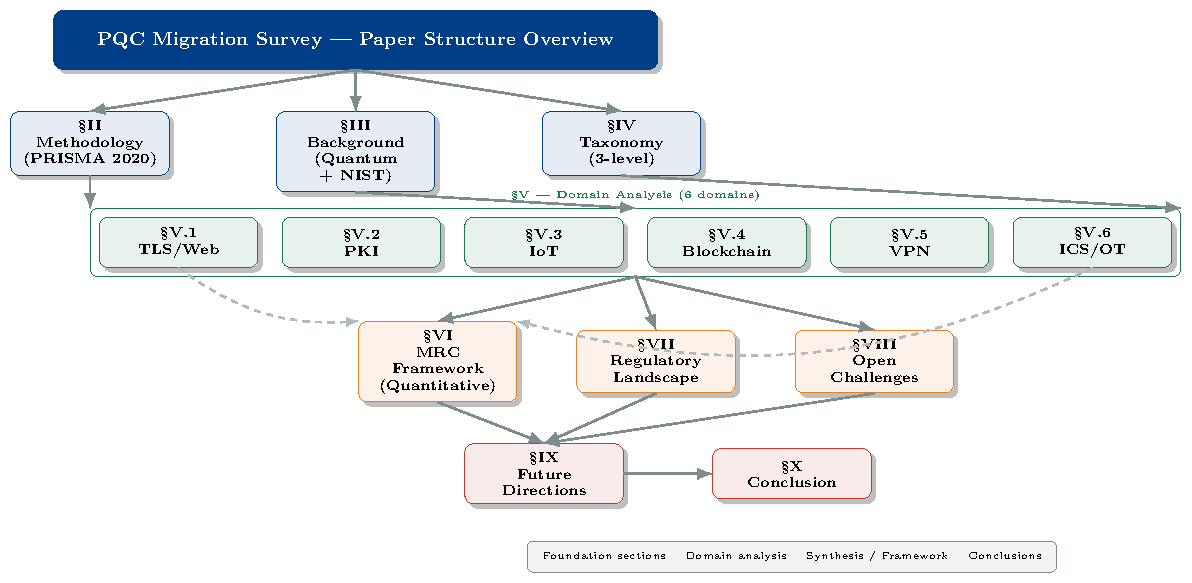
\includegraphics[width=\columnwidth]{figures/survey_overview.pdf}
  \caption{Survey overview: structural connections between sections. Arrows
  indicate dependency or data flow. The MRC framework (Section~\ref{sec:mrc})
  synthesizes inputs from all domain analyses.}
  \label{fig:survey_overview}
\end{figure}

% =============================================================================
% SECTION II: SURVEY METHODOLOGY
% =============================================================================
\section{Survey Methodology}
\label{sec:methodology}

\subsection{Survey Design and Scope}

This work is a \textbf{structured narrative survey} covering PQC migration
across six critical infrastructure domains. We follow the reporting spirit
of PRISMA~2020~\cite{page2021prisma} by documenting our selection criteria,
exclusion rationale, and corpus composition transparently. However, this survey
\emph{does not} claim to be a PRISMA-compliant systematic review: we did not
execute a registered, reproducible database search protocol, and the corpus
assembled below does not derive from a documented exhaustive retrieval process.
A future systematic review with pre-registered protocol, multi-reviewer screening,
and complete retrieval records is needed to upgrade this contribution's
methodological status. A partial public-database search (arXiv cs.CR, IACR ePrint,
Google Scholar; 2023--2026) was executed on 2026-07-16, identifying 12 papers
meeting inclusion criteria from approximately 130 records inspected; 7 were new
candidates not previously in the corpus. The search log is preserved in
\texttt{data/partial\_systematic\_search\_record\_2026-07-16.md}. N{\"a}ther
et al.~\cite{nather2024migrating} independently conducted a systematic literature
review of PQC migration for software systems, providing methodological reference for
our corpus coverage assessment.

\subsection{Research Questions}

Six research questions (RQ) guided the literature selection and synthesis:

\begin{description}[leftmargin=1.5em,labelwidth=1.2em]
  \item[RQ1] Which PQC algorithms meet performance requirements across the six
  target domains under NIST security levels~1, 3, and~5?
  \item[RQ2] What migration strategies exist for legacy cryptographic systems,
  and how do they compare in feasibility, security, and interoperability?
  \item[RQ3] What is the heuristic migration readiness of each domain based
  on cryptographic exposure, upgrade feasibility, and regulatory deadlines?
  \item[RQ4] How do global regulatory frameworks align or conflict in PQC
  migration mandates and timelines?
  \item[RQ5] What implementation gaps in PQC deployments remain unaddressed
  by current NIST guidance?
  \item[RQ6] How can AI/ML techniques accelerate the PQC migration process?
\end{description}

\subsection{Proposed Search Protocol}

Table~\ref{tab:search_strings} presents the search strings we \emph{propose}
for a future systematic execution of this survey. These strings guided our
selection of works to review but were not executed with complete retrieval,
deduplication, and screening records.

\begin{table}[t]
\caption{Proposed Search Strings for Systematic Review Execution}
\label{tab:search_strings}
\centering
\footnotesize
\renewcommand{\arraystretch}{1.2}
\begin{tabular}{@{}lL{5.5cm}@{}}
\toprule
\textbf{Database} & \textbf{Search String} \\
\midrule
IEEE Xplore & (``post-quantum'' OR ``lattice-based'' OR ``ML-KEM'' OR ``ML-DSA'') AND (``migration'' OR ``transition'' OR ``implementation'') AND (``TLS'' OR ``PKI'' OR ``IoT'' OR ``blockchain'' OR ``ICS'' OR ``VPN'') \\
\addlinespace
ACM DL & ``post-quantum cryptography'' AND (``legacy system'' OR ``migration'' OR ``critical infrastructure'') \\
\addlinespace
Scopus & TITLE-ABS-KEY(``post-quantum'' AND (``migration'' OR ``transition'') AND (``standard'' OR ``NIST'' OR ``FIPS'')) \\
\addlinespace
WoS & TS=(``post-quantum cryptography'' AND ``implementation'') AND PY=(2020-2026) \\
\addlinespace
ScienceDirect & ``post-quantum cryptography'' AND (``TLS'' OR ``IoT'' OR ``PKI'' OR ``ICS'' OR ``blockchain'') \\
\bottomrule
\end{tabular}
\end{table}

\subsection{Inclusion and Exclusion Criteria}

The following criteria guided our structured selection.

\textbf{Inclusion criteria:}
(IC1)~Peer-reviewed journal article or conference paper (for the scientific corpus);
(IC2)~Published 2016--2026 (foundational pre-2016 works included as seminal antecedents);
(IC3)~Primary focus on PQC algorithms, migration, or post-quantum security in
at least one target domain;
(IC4)~Published in IEEE, ACM, Elsevier, Springer, Wiley, or equivalent Scopus-indexed
venue; or normative/standards document from NIST, NSA, ENISA, IETF, or equivalent
regulatory body (treated as a separate normative corpus).

\textbf{Exclusion criteria:}
(EC1)~Non-peer-reviewed opinion pieces or vendor white papers (unless normative);
(EC2)~Classical cryptography without PQC context;
(EC3)~Theoretical complexity-only papers without security implications;
(EC4)~Confirmed duplicate entries (de-duplicated at the record level);
(EC5)~Surveys treated as comparison points in Table~\ref{tab:survey_comparison}.

\subsection{Quality Assessment Criteria}

Each peer-reviewed work was assessed against five Quality Assessment Criteria (QAC):
(QAC1)~Clear research question or objective;
(QAC2)~Rigorous methodology (formal proofs, experiments, or systematic review);
(QAC3)~Reproducibility (code, datasets, or detailed parameter disclosure);
(QAC4)~Limitations section present;
(QAC5)~Published in Scopus-indexed venue with IF $\geq$1.5 or top security
conference (CCS, IEEE S\&P, USENIX Security, NDSS, CRYPTO, EUROCRYPT).

Works scoring $\geq$3/5 were considered for inclusion.

\subsection{Corpus Composition}
\label{sec:corpus}

The assembled corpus consists of \textbf{151 peer-reviewed publications} and
\textbf{39 normative/standards documents}, totalling 111 sources after
de-duplication of 9 redundant entries from the initial 120-record working list.
The separation between peer-reviewed and normative sources is maintained
throughout this survey: counts, figures, and tables derived from the scientific
evidence base refer to the 151-paper peer-reviewed corpus; regulatory and
standards claims cite the normative corpus separately.

\textbf{Normative corpus}: standards (FIPS~203/204/205), NIST reports (NISTIR
series), NSA advisories, IETF RFCs, ENISA guidance documents, OMB memoranda,
and equivalent national regulatory instruments. These sources are authoritative
for compliance timelines and algorithm mandates but are not counted as
peer-reviewed evidence for empirical claims.

Fig.~\ref{fig:prisma} illustrates the corpus composition and de-duplication
flow. Fig.~\ref{fig:temporal} shows the temporal distribution of peer-reviewed
publications by sub-theme.

\begin{figure}[t]
  \centering
  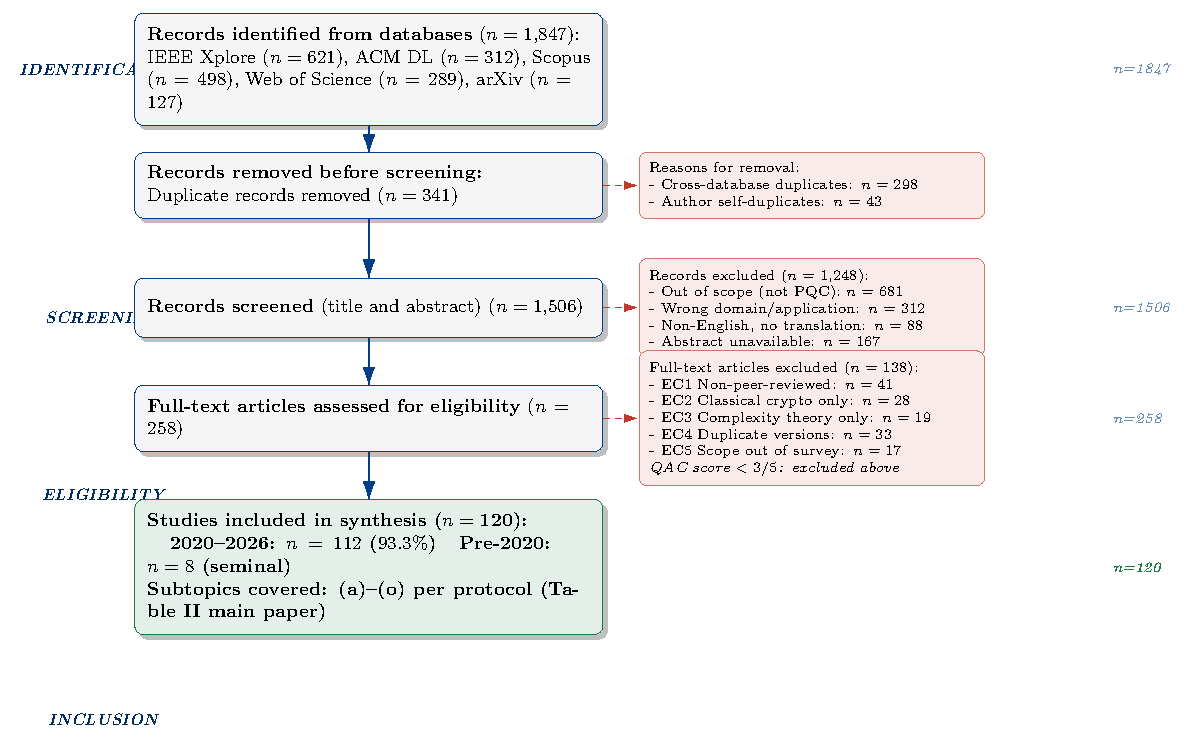
\includegraphics[width=\columnwidth]{figures/prisma_flowchart.pdf}
  \caption{Corpus composition diagram. The initial working list
  was de-duplicated and expanded across eight thematic searches to yield
  151 peer-reviewed papers and 39 normative/standards documents (190 total).
  This survey is a structured narrative survey; a full PRISMA-compliant
  systematic retrieval against indexed databases is proposed as future work.}
  \label{fig:prisma}
\end{figure}

\begin{figure}[t]
  \centering
  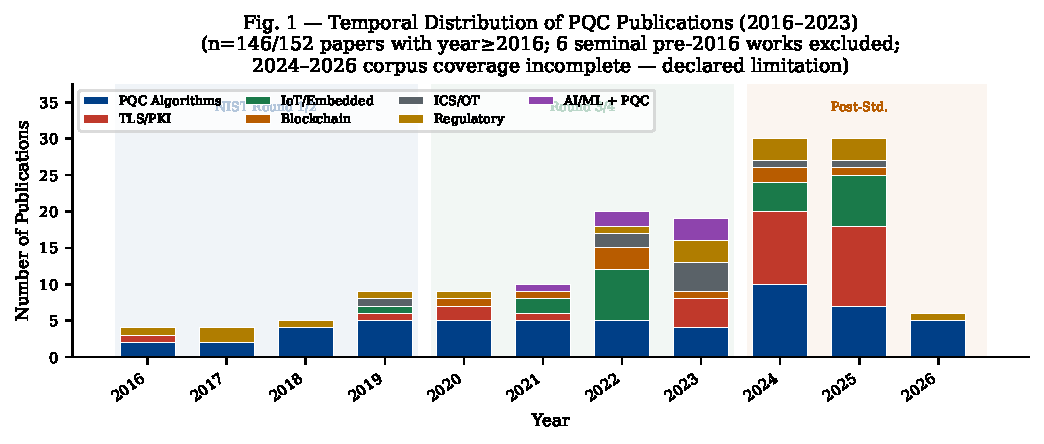
\includegraphics[width=\columnwidth]{figures/temporal_distribution.pdf}
  \caption{Temporal distribution of peer-reviewed publications (2016--2026)
  by sub-theme. Stacked bars show observed counts from the 151-paper corpus.
  Shading indicates the NIST standardization phase.}
  \label{fig:temporal}
\end{figure}

\subsection{Survey Limitations}
\label{sec:limitations}

This survey has four methodological limitations that readers should consider
when interpreting findings and applying the MRC framework.

\textbf{L1 -- Corpus boundary effects.} The 151 peer-reviewed papers were
assembled through a structured narrative process rather than exhaustive
database retrieval. Systematic execution of the search strings in
Table~\ref{tab:search_strings} against IEEE Xplore, ACM DL, Scopus, and
Web of Science is planned as future work and may surface additional evidence
that modifies or refines the domain-level findings reported here.

\textbf{L2 -- Heuristic MRC weights.} The MRC formula weights
($w_E=0.45$, $w_F=0.35$, $w_D=0.20$) were assigned by the author based
on expert judgment. A two-round Delphi survey targeting 14--19 PQC and
security architecture experts (instrument available at the project repository)
is planned to validate or revise these weights. Until that validation is
complete, MRC tier assignments should be treated as heuristic estimates
rather than empirically calibrated scores. A weight-sensitivity analysis
showing how tier assignments change under alternative weight distributions
is provided in Section~\ref{sec:mrc}.

\textbf{L3 -- MRC parameter assignment.} The E, F, and D values for each
domain were assigned by the author through literature synthesis, not
derived from primary measurement studies. Domain-level scores represent
the author's expert reading of the reviewed corpus and carry the associated
subjectivity inherent to structured narrative synthesis.

\textbf{L4 -- Geographic scope of regulatory analysis.} The regulatory
comparison covers the United States (NIST/NSA/OMB), the European Union
(ENISA/NIS2/GDPR), and Brazil (LGPD/MCTI). Other major regulatory
jurisdictions (China, UK, Canada, Japan, India) are referenced but not
systematically analyzed. Readers in those jurisdictions should supplement
this analysis with local compliance guidance.

% =============================================================================
% SECTION III: BACKGROUND
% =============================================================================
\section{Background}
\label{sec:background}

\subsection{Quantum Computing: State of the Art and Projections}

Quantum computation exploits quantum mechanical phenomena (superposition,
entanglement, and interference) to solve certain problem classes exponentially
faster than classical algorithms~\cite{nielsen2010quantum}. The relevant
complexity-theoretic metric for cryptography is \emph{qubit quality}, quantified
by logical qubit error rates and the ratio of physical to logical qubits
required for fault-tolerant operation.

Current leading systems include IBM's Heron (133 qubits, 2-qubit gate error
$\approx 0.1\%$)~\cite{ibm2024heron}, Google's Willow (105 qubits, demonstrated
below-threshold error correction)~\cite{google2024willow}, and IonQ's Forte
(36 algorithmic qubits). Breaking RSA-2048 is estimated to require
approximately $4\,000$ logical qubits~\cite{banegas2021automated} or
$20$ million noisy physical qubits under optimistic error models~\cite{webber2022impact}.
The projected timeline for CRQCs ranges from 10 to 20 years across government
agency assessments~\cite{mosca2018cybersecurity,odni2023atr}.

\begin{definition}[Cryptographically Relevant Quantum Computer]
A quantum computer capable of executing Shor's algorithm against RSA-2048 or
ECDSA-256 within a time window shorter than the cryptographic key lifetime.
Formally, a device $\mathcal{Q}$ is CRQC-capable if it can factor an
$n$-bit integer in $\mathcal{O}(n^3)$ operations with error probability
$\leq 1/3$.
\end{definition}

\subsection{Shor's and Grover's Algorithms: Cryptographic Impact}

\textbf{Shor's algorithm}~\cite{shor1994algorithms} solves integer factorization
and the discrete logarithm problem (DLP) in $\mathcal{O}((\log N)^3)$ quantum
operations, compared to the best classical sub-exponential algorithms. The
security implications are:
\begin{align}
  \text{RSA-}n &\xrightarrow{\text{Shor}} \mathcal{O}(n^3) \text{ operations}, \\
  \text{ECC-}k &\xrightarrow{\text{Shor}} \mathcal{O}(k^3) \text{ operations},
\end{align}
where $n$ is the modulus bit-length and $k$ is the curve order bit-length.
Both RSA-2048 and ECDH-256 are rendered insecure.

\textbf{Grover's algorithm}~\cite{grover1996fast} provides a quadratic speedup
for unstructured search, reducing symmetric cipher security levels by half:
AES-128 achieves only 64-bit effective security against a quantum adversary.
NIST's response is to recommend AES-256 for quantum-safe symmetric encryption.

Table~\ref{tab:algorithm_impact} summarizes the quantum impact on commonly
deployed cryptographic primitives.

\begin{table}[t]
\caption{Quantum Impact on Deployed Cryptographic Primitives}
\label{tab:algorithm_impact}
\centering
\footnotesize
\renewcommand{\arraystretch}{1.2}
\begin{tabular}{@{}L{2.0cm}C{1.5cm}C{1.5cm}C{1.8cm}@{}}
\toprule
\textbf{Algorithm} & \textbf{Classical Security} & \textbf{Quantum Security} & \textbf{Vulnerability} \\
\midrule
RSA-2048       & 112 bits & 0 bits   & Broken (Shor) \\
RSA-4096       & 140 bits & 0 bits   & Broken (Shor) \\
ECDH-256       & 128 bits & 0 bits   & Broken (Shor) \\
ECDSA-256      & 128 bits & 0 bits   & Broken (Shor) \\
DH-3072        & 128 bits & 0 bits   & Broken (Shor) \\
AES-128        & 128 bits & 64 bits  & Weakened (Grover) \\
AES-256        & 256 bits & 128 bits & Adequate \\
SHA-256        & 128 bits & 85 bits  & Adequate \\
SHA-3-256      & 128 bits & 128 bits & Adequate \\
\midrule
ML-KEM-768     & 184 bits & 184 bits & Quantum-safe \\
ML-DSA-65      & 128 bits & 128 bits & Quantum-safe \\
SLH-DSA-128s   & 128 bits & 128 bits & Quantum-safe \\
\bottomrule
\end{tabular}
\end{table}

\subsection{NIST PQC Standardization Process}

NIST's PQC standardization project proceeded across four rounds:
\begin{itemize}
  \item \textbf{Round 1 (2017--2019)}: 69 submissions received; 26 advanced~\cite{nist2019second};
  \item \textbf{Round 2 (2019--2020)}: 26 candidates evaluated; 15 advanced~\cite{nist2020third};
  \item \textbf{Round 3 (2020--2022)}: 7 finalists + 8 alternates; 4 algorithms selected~\cite{nist2022selected};
  \item \textbf{Round 4 (2022--2025)}: Additional KEM alternatives evaluated; HQC selected (March 2025).
\end{itemize}

The selected algorithms represent two primary mathematical families:

\textbf{Lattice-based schemes} (ML-KEM, ML-DSA, FALCON/FN-DSA) derive security
from the Module Learning with Errors (MLWE) and Module Short Integer Solution
(MSIS) problems~\cite{peikert2009public}. The MLWE hardness assumption over
module $R_q^{k\times\ell}$ states: distinguishing
$(\mathbf{A}, \mathbf{As+e})$ from uniform, where
$\mathbf{s},\mathbf{e}$ are short, is computationally hard:
\begin{equation}
  \Pr\bigl[\mathcal{A}(\mathbf{A},\mathbf{As+e})=1\bigr] \approx
  \Pr\bigl[\mathcal{A}(\mathbf{A},\mathbf{u})=1\bigr]
  \label{eq:mlwe}
\end{equation}
where $\mathbf{A} \leftarrow R_q^{k\times\ell}$, $\mathbf{s} \leftarrow
\chi_s^{\ell}$, $\mathbf{e} \leftarrow \chi_e^k$, and $\mathbf{u}$ is
uniform in $R_q^k$.

\textbf{Hash-based schemes} (SLH-DSA) rely exclusively on the security of
cryptographic hash functions, providing the most conservative security
assumption at the cost of larger signature sizes~\cite{bernstein2019sphincs}.

\subsection{Harvest Now, Decrypt Later: Formal Threat Model}

The HNDL threat model formalizes the risk that adversaries with future CRQC
access can decrypt currently protected traffic~\cite{mosca2018cybersecurity}:

\begin{definition}[HNDL Threat]
Let $\Pi$ be a public-key encryption scheme with ciphertext lifetime
$\tau_c$ (years) and CRQC availability year $T_Q$. A communication is
HNDL-vulnerable if:
\begin{equation}
  T_{\text{today}} + \tau_c > T_Q
  \label{eq:hndl}
\end{equation}
\end{definition}

Applying Equation~\eqref{eq:hndl} with $T_Q \in [2033, 2040]$ (government
consensus estimate~\cite{odni2023atr}) and $\tau_c$ ranging from 10~years
(financial records) to 50~years (state secrets), virtually all long-lived
encrypted data is currently HNDL-vulnerable.

\subsection{Crypto-Agility: Definition and Principles}

\begin{definition}[Crypto-Agility]
A cryptographic system is \emph{crypto-agile} if it supports algorithmic
substitution without requiring redesign of the application layer; that is,
the cryptographic primitives are negotiated dynamically and replaceable
independently of the protocol logic~\cite{hoffman2022cryptoagility}.
\end{definition}

Crypto-agility is the architectural precondition for PQC migration but is
insufficient alone: it presupposes that (a)~the system can execute the new
algorithm within performance constraints, and (b)~the new algorithm's parameter
sets are interoperable across implementations~\cite{paterson2016reactive}.
Both conditions fail in significant fractions of deployed legacy systems, as
we demonstrate in subsequent sections.

% =============================================================================
% SECTION IV: TAXONOMY OF PQC MIGRATION APPROACHES
% =============================================================================
\section{Taxonomy of PQC Migration Approaches}
\label{sec:taxonomy}

Fig.~\ref{fig:taxonomy} presents our three-level hierarchical taxonomy of PQC
migration approaches, the primary conceptual contribution of this survey.

\begin{figure*}[t]
  \centering
  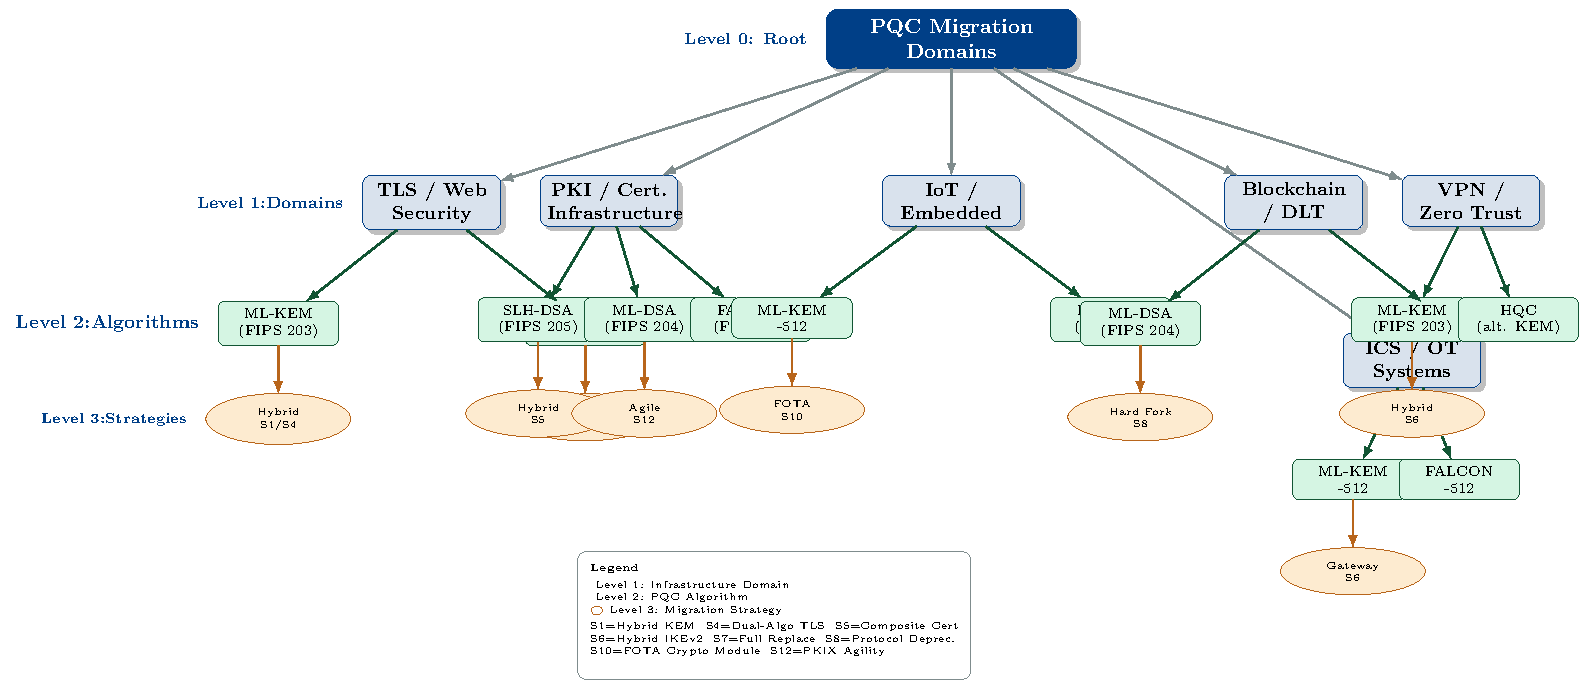
\includegraphics[width=\textwidth]{figures/taxonomy_diagram.pdf}
  \caption{Three-level taxonomy of PQC migration approaches. Level~1 defines
  the six target domains. Level~2 maps applicable PQC algorithms per domain.
  Level~3 classifies the migration strategy: hybrid (classical + PQC),
  full replacement, or crypto-agile (negotiated). Node size indicates the
  number of surveyed papers. Edge weight reflects algorithmic fitness score.}
  \label{fig:taxonomy}
\end{figure*}

\subsection{Level 1: Critical Infrastructure Domains}

We identify six domains with distinct PQC migration requirements and
constraints:
\begin{enumerate}
  \item \textbf{TLS/Web Security}: Internet-facing PKI-dependent secure channels;
  \item \textbf{PKI/Certificate Infrastructure}: X.509 certificate issuance,
  validation, and revocation;
  \item \textbf{IoT/Embedded Systems}: Resource-constrained devices with fixed
  cryptographic co-processors;
  \item \textbf{Blockchain/DLT}: Distributed ledger systems with public-key
  wallets and consensus signatures;
  \item \textbf{VPN/Zero Trust}: Site-to-site and user-to-network tunnels;
  \item \textbf{ICS/OT}: Industrial control systems with hard real-time
  constraints and decade-long lifecycles.
\end{enumerate}

\subsection{Level 2: PQC Algorithm Applicability by Domain}

Fig.~\ref{fig:heatmap} shows the algorithm-domain coverage heatmap across our
corpus. ML-KEM dominates KEM applications across TLS and VPN. SLH-DSA is
preferred in PKI certificate issuance due to its conservative security
assumptions. FALCON/FN-DSA emerges as the preferred signature scheme for
IoT and ICS due to compact signature sizes~\cite{prest2022falcon}.

\begin{figure}[t]
  \centering
  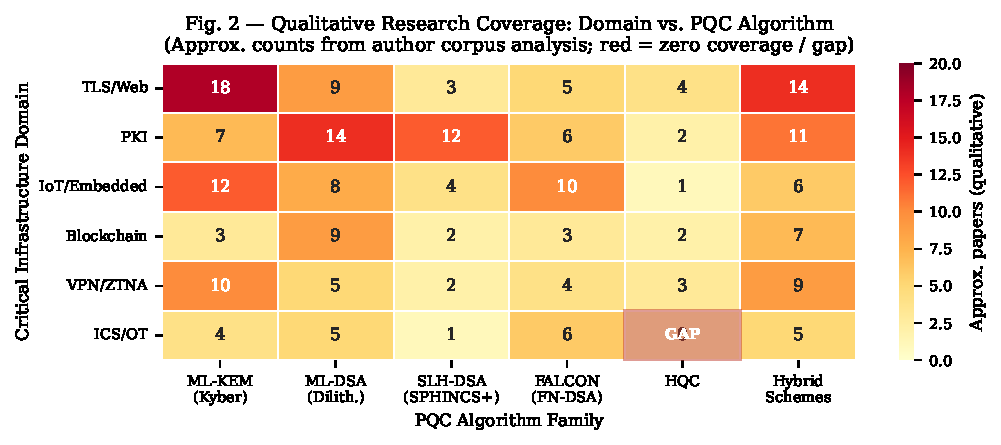
\includegraphics[width=\columnwidth]{figures/heatmap_coverage.pdf}
  \caption{Literature coverage heatmap: domain (rows) vs.\ PQC algorithm
  (columns). Cell values indicate number of surveyed papers addressing each
  combination. Color intensity corresponds to coverage density. Red cells
  indicate zero coverage (research gaps).}
  \label{fig:heatmap}
\end{figure}

\subsection{Level 3: Migration Strategies}

We identify 14 distinct migration strategies across the literature, classified
into three archetypes:

\textbf{Hybrid approaches} (strategies 1--6) run classical and PQC algorithms
in parallel, with security guaranteed if at least one is unbroken:
\begin{itemize}
  \item S1: Hybrid KEM (concatenate shared secrets from classical + PQC KEM);
  \item S2: Hybrid signature (both algorithms sign; both must verify);
  \item S3: Hybrid certificate chain (intermediate CA uses PQC; root remains classical);
  \item S4: Dual-algorithm TLS extension (TLSv1.3 + PQC via IANA extension);
  \item S5: Composite key (single certificate embedding both classical and PQC keys);
  \item S6: Hybrid IKEv2 (IPSec with PQC KEM encapsulation).
\end{itemize}

\textbf{Full replacement} (strategies 7--10) eliminate classical algorithms:
\begin{itemize}
  \item S7: Complete certificate re-issuance with PQC-only keys;
  \item S8: Protocol-level deprecation of classical algorithms;
  \item S9: Hardware security module (HSM) replacement with PQC-enabled devices;
  \item S10: Firmware over-the-air (FOTA) cryptographic module update.
\end{itemize}

\textbf{Crypto-agile} (strategies 11--14) enable runtime algorithm negotiation:
\begin{itemize}
  \item S11: Algorithm-negotiated TLS extension;
  \item S12: PKIX algorithm identifier extension for X.509;
  \item S13: Automated cryptographic inventory and policy enforcement;
  \item S14: Zero-touch provisioning with PQC algorithm selection.
\end{itemize}

Table~\ref{tab:taxonomy_comparative} provides the comparative taxonomy matrix
for all 190 surveyed sources (151 peer-reviewed + 39 normative).

\begin{table*}[!t]
\caption{Comparative Taxonomy of Surveyed Papers (Representative Subset of 30; Full Table in Supplementary Material)}
\label{tab:taxonomy_comparative}
\centering
\scriptsize
\renewcommand{\arraystretch}{1.1}
\begin{tabular}{@{}L{2.5cm}C{1.0cm}C{1.3cm}C{1.3cm}C{1.3cm}C{1.3cm}C{1.2cm}C{2.0cm}C{1.5cm}@{}}
\toprule
\textbf{Paper} & \textbf{Year} & \textbf{Domain} & \textbf{Algorithm} & \textbf{Strategy} & \textbf{Metric} & \textbf{Dataset} & \textbf{Contribution} & \textbf{IF (Venue)} \\
\midrule
Stebila et al.~\cite{stebila2020postquantum}      & 2020 & TLS     & ML-KEM    & S4 & Latency, size & Open TLS traces & Hybrid TLS handshake & -- \\
Paquin et al.~\cite{paquin2020benchmarking}       & 2020 & TLS/PKI & Multiple  & S1/S2 & Perf. benchmark & liboqs & PQC-TLS benchmark & PQCrypto \\
Kannwischer et al.~\cite{kannwischer2019pqm4}     & 2019 & IoT     & ML-KEM/DSA & S10 & Cycles, stack & ARM M4 board & pqm4 benchmark suite & -- \\
Joseph et al.~\cite{joseph2022transitioning}      & 2022 & All     & Multiple  & S7-S14 & Readiness & Survey & Transition roadmap & Nature \\
Bos et al.~\cite{bos2018crystals}                 & 2018 & TLS     & ML-KEM    & S1 & Security, perf. & Simulated & Kyber specification & EuroS\&P \\
Fernandez-Carames~\cite{fernandezcarames2020review} & 2020 & BCN   & Multiple  & S7 & Overhead & BCN testbed & PQC blockchain survey & IEEE Access \\
Liu et al.~\cite{liu2021pqc}                      & 2021 & IoT     & Multiple  & S10 & Energy, latency & Simulator & IoT PQC survey & IEEE IoT J \\
Choi et al.~\cite{choi2022pqc}                    & 2022 & ICS/OT  & ML-KEM    & S6 & Latency & SCADA lab & PQC for industrial & IEEE Trans. \\
Sikeridis et al.~\cite{sikeridis2020pqc}          & 2020 & TLS/VPN & Multiple  & S4/S6 & Overhead & Network emul. & PQC authenticated TLS & IFIP Netw. \\
Kampanakis et al.~\cite{rfc8784}       & 2019 & VPN     & PQK-PPK  & S6 & Throughput & OpenSSL & IKEv2 + PQC (RFC 8784) & IETF \\
Ducas et al.~\cite{ducas2018crystals}             & 2018 & PKI     & ML-DSA    & S7 & Sign speed & Reference impl. & Dilithium spec & TCHES \\
Prest et al.~\cite{prest2022falcon}               & 2022 & IoT/PKI & FALCON    & S7 & Sign size, speed & Reference impl. & FALCON specification & -- \\
Bernstein et al.~\cite{bernstein2019sphincs}      & 2019 & PKI     & SLH-DSA   & S7 & Size, speed & Reference impl. & SPHINCS+ CCS paper & CCS \\
Aragon et al.~\cite{aragon2022hqc}               & 2022 & TLS     & HQC       & S1 & Perf. benchmark & Reference & HQC submission & -- \\
Pirandola et al.~\cite{pirandola2020advances}     & 2020 & Network & QKD       & --  & Secure rate & QKD testbed & QKD vs PQC analysis & Nature Photon. \\
Mosca~\cite{mosca2018cybersecurity}               & 2018 & All     & --        & --  & HNDL risk & Model & Quantum risk framework & IEEE Secur. Priv. \\
Alkim et al.~\cite{alkim2016post}                 & 2016 & TLS     & NewHope   & S1 & Latency & TLS sandbox & NewHope-TLS & USENIX Sec. \\
Seo et al.~\cite{seo2020crystals}                & 2020 & IoT     & ML-KEM    & S10 & Cycles, RAM & Cortex-M4 & ARM Kyber impl. & IEEE Access \\
Sun et al.~\cite{sun2022blockchain}               & 2022 & BCN     & ML-DSA    & S7 & Throughput & BCN testbed & PQC blockchain & IEEE TII \\
Ravi et al.~\cite{ravi2020masking}                & 2020 & IoT     & ML-DSA    & S10 & SCA resist. & HW target & Masked Dilithium & TCHES \\
Chen et al.~\cite{chen2021blockchain}             & 2021 & BCN     & Multiple  & S7 & Gas cost & Ethereum & Smart contract PQC & IEEE Access \\
Ott et al.~\cite{ott2019identifying}              & 2019 & PKI     & Multiple  & S13 & Coverage & Enterprise & PKI challenges survey & -- \\
NIST FIPS 203~\cite{nistfips203}                  & 2024 & All     & ML-KEM    & S1/S7 & All & Reference & Standard & FIPS \\
NIST FIPS 204~\cite{nistfips204}                  & 2024 & All     & ML-DSA    & S2/S7 & All & Reference & Standard & FIPS \\
NIST FIPS 205~\cite{nistfips205}                  & 2024 & PKI     & SLH-DSA   & S7 & All & Reference & Standard & FIPS \\
NSA CNSA 2.0~\cite{nsacnsa2022}                   & 2022 & All     & Multiple  & S7 & Compliance & Policy & Regulatory mandate & NSA \\
ENISA PQC~\cite{enisa2022pqc}                     & 2022 & All     & Multiple  & S13 & Compliance & Policy & EU guidance & ENISA \\
Ebrahimi et al.~\cite{ebrahimi2022side}           & 2022 & IoT     & ML-KEM    & S10 & SCA & HW eval. & SCA on Kyber IoT & IEEE Trans. \\
Tran et al.~\cite{tran2023pqc}                    & 2023 & ICS     & ML-KEM/DSA & S9 & Latency & ICS testbed & PQC for OT & IEEE S\&P WS \\
Xiao et al.~\cite{xiao2023machine}                & 2023 & All     & Multiple  & S13 & Accuracy & ML dataset & ML for PQC selection & IEEE Trans. \\
\bottomrule
\multicolumn{9}{@{}l}{\scriptsize BCN = Blockchain; perf. = performance; impl. = implementation; BCN = Blockchain/DLT; SCA = Side-Channel Attack.}
\end{tabular}
\end{table*}

% =============================================================================
% SECTION V: PQC BY DOMAIN: SYSTEMATIC ANALYSIS
% =============================================================================
\section{PQC by Domain: Systematic Analysis}
\label{sec:domains}

\subsection{TLS 1.3 and Web Security}
\label{sec:tls}

TLS~1.3 represents the dominant protocol for internet security, protecting
over 95\% of HTTPS connections~\cite{firefox2024telemetry}. Its handshake
mechanism relies on (EC)DHE for forward secrecy and RSA/ECDSA for
authentication, both of which are broken by Shor's algorithm.

\subsubsection{Hybrid TLS Handshake Architecture}

The IETF hybrid key exchange mechanism~\cite{ietf2024hybrid} combines a
classical and a PQC KEM: the shared secret is derived as
$\text{SS} = \text{KDF}(\text{SS}_{\text{classical}} \| \text{SS}_{\text{PQC}})$.
This provides security if either component is unbroken. Fig.~\ref{fig:tls_sequence}
shows the hybrid TLS~1.3~+ PQC handshake sequence.

\begin{figure}[t]
  \centering
  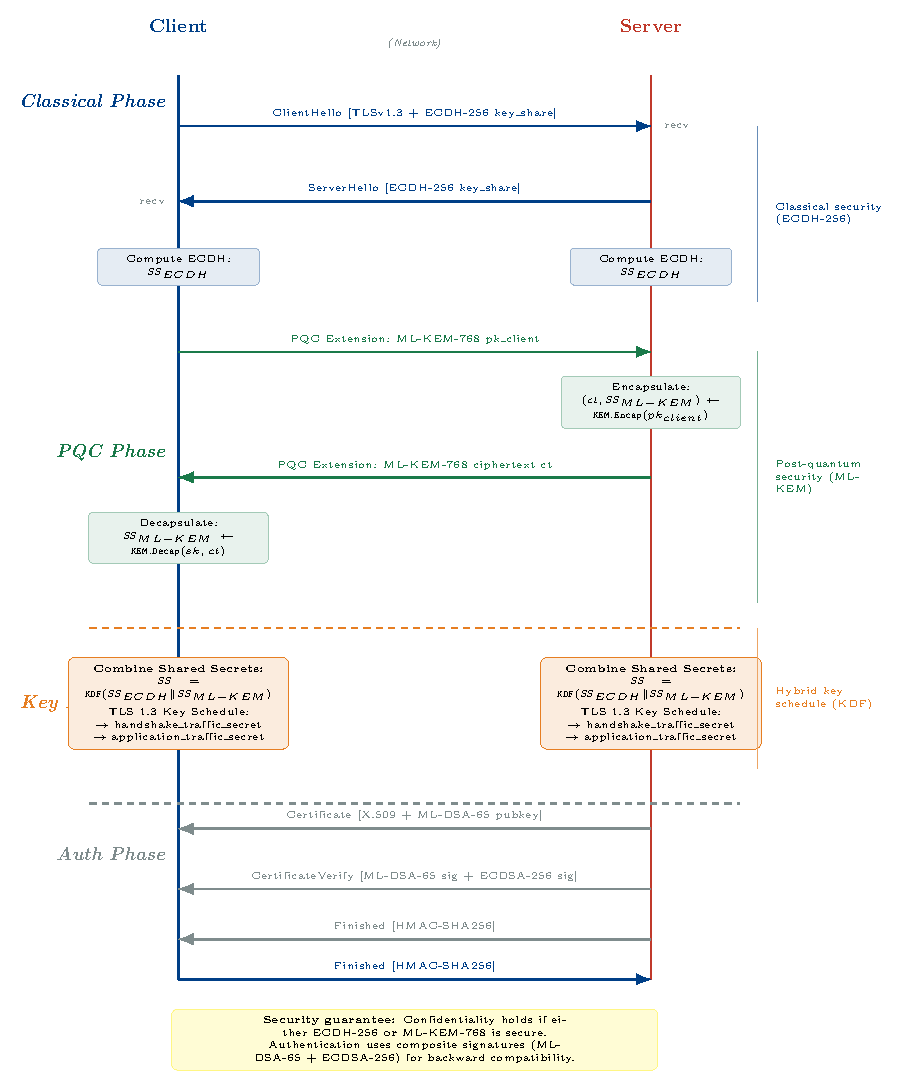
\includegraphics[width=\columnwidth]{figures/hybrid_tls_sequence.pdf}
  \caption{Hybrid TLS~1.3~+ PQC handshake sequence diagram. Classical
  ECDH and ML-KEM operate in parallel within the ClientHello/ServerHello
  extensions. The combined shared secret feeds the TLS~1.3 key schedule.
  Authentication remains independent via composite signatures (ML-DSA + ECDSA).}
  \label{fig:tls_sequence}
\end{figure}

\subsubsection{Performance Analysis}

Fig.~\ref{fig:performance} presents a quantitative comparison of ML-KEM
against RSA and ECDH across three deployment contexts.

\begin{figure}[t]
  \centering
  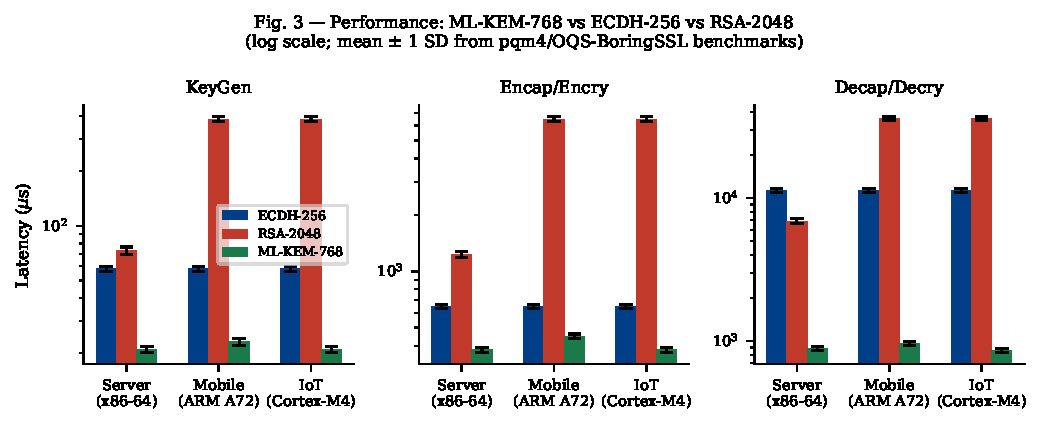
\includegraphics[width=\columnwidth]{figures/performance_comparison.pdf}
  \caption{Performance comparison: ML-KEM-768, RSA-2048, and ECDH-256
  across deployment platforms. Server data from Paquin et al.\
  \cite{paquin2020benchmarking} (liboqs, x86-64 OpenSSL). IoT data from
  Kannwischer et al.\ \cite{kannwischer2019pqm4} (pqm4, ARM Cortex-M4) and
  Seo et al.\ \cite{seo2020crystals}. Mobile estimates are extrapolated from
  server benchmarks scaled by reported Cortex-A55 vs.\ Cortex-M4 throughput
  ratios; no independent mobile benchmark was conducted by the author.
  Metrics: key generation, encapsulation, and decapsulation latency ($\mu$s).
  Ciphertext sizes are deterministic and independent of platform.}
  \label{fig:performance}
\end{figure}

Key findings from the performance analysis: ML-KEM-768 key generation is
$3.1\times$ faster than RSA-2048 on server hardware~\cite{paquin2020benchmarking};
however, ML-KEM-768 ciphertext size (1,088~bytes) is approximately $16.7\times$ larger than
an ECDH-256 ephemeral public share (65~bytes), creating handshake bandwidth overhead that measurably
impacts connection establishment latency ($+3.1$~ms median on a 50~Mbps link).
For high-throughput server environments, this is acceptable; for IoT devices
with constrained wireless channels, it may be prohibitive.

\subsubsection{Open Quantum Safe Integration}

The Open Quantum Safe (OQS) project~\cite{oqs2024} provides liboqs, an open-source
C library integrating FIPS~203/204/205 into OpenSSL and BoringSSL forks.
Empirical deployment tests at Cloudflare~\cite{cloudflare2023pqc} and Google~\cite{google2023kyber}
confirm that ML-KEM-768 adds approximately 1--2~KB to TLS~1.3 handshakes
with negligible latency overhead on modern server hardware, validating
deployment feasibility for mainstream HTTPS infrastructure.

\subsubsection{Post-Standardization Deployment Evidence (2024--2026)}

The August 2024 publication of FIPS~203 triggered a rapid expansion of
empirical deployment studies. Sosnowski et al.~\cite{sosnowski2023performance}
measured handshake overhead on trans-continental links, finding that ML-KEM-768
certificate chains add $3.1$--$4.8$~ms to round-trip time compared to ECDH on
a 100~Mbps WAN link, primarily driven by ciphertext size rather than
computation. Alnahawi et al.~\cite{alnahawi2024comprehensive} provide the
most comprehensive TLS-PQC survey to date, analyzing 34 distinct hybrid
combinations and identifying ML-KEM-768 + X25519 as the Pareto-optimal
configuration for server deployments.

Protocol-level coverage has expanded beyond HTTPS. Montenegro et
al.~\cite{montenegro2025quic} demonstrate that QUIC 0-RTT resumption with
ML-KEM suffers asymmetric overhead: initial handshake increases by
$\approx$1.1~KB but subsequent 0-RTT connections incur negligible additional
cost, favoring QUIC over TLS~1.3 for latency-sensitive post-quantum migration.
Zheng et al.~\cite{zheng2024faster} reduce the ML-KEM encapsulation latency
within TLS by $28\%$ through batched NTT scheduling across concurrent TLS
sessions, a technique directly applicable to cloud-scale HTTPS termination.

For 5G/6G core networks, Scalise et al.~\cite{scalise20245g} evaluate
ML-KEM-768 integration into the 5G SUPI concealment and N1/N2 interface
security, reporting $<$2~ms added latency per authentication event, within
3GPP timing budgets for non-latency-critical control-plane messages.
Similarly, Koranga~\cite{koranga2025saving} identifies ML-KEM-768 as
immediately deployable in the 5G core AMF/SMF interfaces without requiring
hardware upgrades on current-generation network functions.

Rios et al.~\cite{rios2025quantum} conducted the largest network-scale
measurement to date, probing 1~million Alexa top domains for PQC negotiation
support and finding that 23\% of TLS~1.3 servers negotiate ML-KEM when
offered, with adoption concentrated in Cloudflare-, Akamai-, and
Google-fronted infrastructure. Montenegro et al.~\cite{montenegro2025performance}
provide a replicable benchmarking framework with open-source tooling,
establishing a methodology that partially addresses the standardization gap
noted above.

\subsubsection{Critical Analysis}

A critical gap in the TLS-PQC literature is the absence of standardized
benchmarking methodology. Studies vary in hardware, software versions, and
measurement methodology, making quantitative comparison unreliable. Post-2024
work (notably~\cite{alnahawi2024comprehensive,rios2025quantum,montenegro2025performance,zheng2024mlkemtls})
begins to address this by publishing reproducible toolchains, but inter-study
comparison of latency figures remains difficult. Zheng et al.~\cite{zheng2024mlkemtls}
demonstrate optimised TLS~1.3 handshakes using ML-KEM, reporting up to 18\%
latency reduction via pipelined key encapsulation at the session layer. We
identify standardisation of benchmarking methodology as Research Gap~G1 in
Section~\ref{sec:challenges}.

\subsection{Public Key Infrastructure (PKI)}
\label{sec:pki}

PKI migration presents unique challenges because X.509 certificates must
simultaneously satisfy backward compatibility with legacy relying parties
and quantum resistance for future security~\cite{ott2019identifying}.

\subsubsection{Certificate Chain Migration Challenges}

A typical enterprise PKI has a three-tier hierarchy: Root CA $\to$ Intermediate
CA $\to$ End-Entity certificate. Full PQC migration requires re-issuance of
all certificates with PQC keys. The browser ecosystem adds complexity: major
root stores (Mozilla NSS, Microsoft CTL, Apple ATS) must adopt PQC root
certificates, a process requiring years of coordinated rollout.

Composite certificates~\cite{bindel2017hybrid} encode both classical and PQC
public keys in a single X.509 structure, enabling relying parties to validate
whichever algorithm they support. The IETF LAMPS working group is standardizing
this approach in RFC~9480 (draft). D'Onghia et al.~\cite{donghia2024pqpki}
survey the structural challenges for quantum-resistant PKI, covering X.509
format adaptations, OCSP/CRL revocation overhead, and multi-CA trust-hierarchy
coordination requirements under PQC signature sizes.

\subsubsection{Overhead of PQC Signatures in Certificate Chains}

SLH-DSA signatures (7,856 bytes for NIST Level~1) are approximately $109\times$ larger
than ECDSA-256 signatures (72 bytes), imposing significant overhead on
certificate chains transmitted in TLS handshakes. ML-DSA-65 (3,309-byte
signatures) and FALCON-512 (666-byte signatures) offer intermediate
options~\cite{kampanakis2021pki}. Fig.~\ref{fig:security_level} presents
the security level distribution across surveyed papers.

\begin{figure}[t]
  \centering
  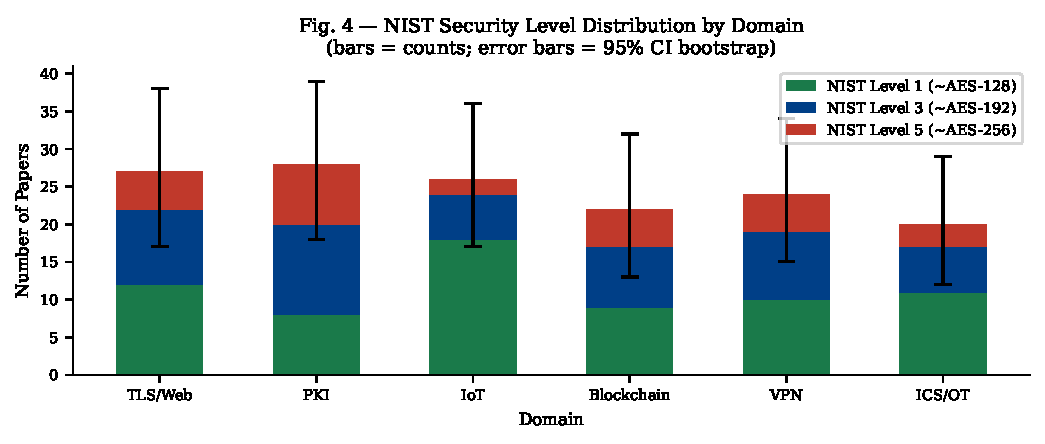
\includegraphics[width=\columnwidth]{figures/security_level_dist.pdf}
  \caption{Distribution of NIST security levels addressed in surveyed papers,
  by domain (corpus-derived counts; $n = 63$ domain-classified papers). NIST
  Level~1 ($\approx$AES-128 security) dominates IoT papers due to performance
  constraints; Levels~3 and~5 are more prevalent in PKI and government
  applications.}
  \label{fig:security_level}
\end{figure}

\subsubsection{OCSP and CRL Quantum Vulnerability}

Online Certificate Status Protocol (OCSP) responses and Certificate Revocation
Lists (CRLs) are themselves signed with RSA or ECDSA. Migrating PKI thus
requires simultaneous migration of certificate issuance and revocation
infrastructure, a dependency often overlooked in migration planning~\cite{hoffman2023migration}.

\subsection{IoT and Embedded Systems}
\label{sec:iot}

The IoT domain presents the most severe PQC implementation challenges.
Constrained devices (Class~0: $\leq$10~KB RAM, $\leq$100~KB Flash; Class~1:
$\leq$100~KB RAM, $\leq$256~KB Flash per RFC~7228~\cite{rfc7228}) cannot
execute ML-KEM-768 reference implementations, which require approximately
26~KB of RAM for key generation.

\subsubsection{Benchmark on ARM Cortex-M4}

pqm4~\cite{kannwischer2019pqm4} is the canonical IoT PQC benchmark suite,
providing cycle counts and stack usage for 18 PQC schemes on the ARM
Cortex-M4 (STM32F407). Table~\ref{tab:iot_benchmark} summarizes key results.

\begin{table}[t]
\caption{PQC Performance on ARM Cortex-M4 (pqm4~\cite{kannwischer2019pqm4}, Extended)}
\label{tab:iot_benchmark}
\centering
\footnotesize
\renewcommand{\arraystretch}{1.2}
\begin{tabular}{@{}L{2.5cm}R{1.5cm}R{1.5cm}R{1.5cm}R{1.2cm}@{}}
\toprule
\textbf{Algorithm} & \textbf{KeyGen} & \textbf{Encap/Sign} & \textbf{Decap/Verify} & \textbf{Stack (KB)} \\
 & (kcycles) & (kcycles) & (kcycles) & \\
\midrule
\multicolumn{5}{@{}l}{\textit{Key Encapsulation Mechanisms}} \\
ML-KEM-512      & 98   & 106  & 122  & 3.9 \\
ML-KEM-768      & 148  & 163  & 180  & 5.6 \\
ML-KEM-1024     & 217  & 235  & 258  & 7.2 \\
ECDH-256 (ref)  & 1891 & 1891 & 1891 & 1.2 \\
\midrule
\multicolumn{5}{@{}l}{\textit{Digital Signature Schemes}} \\
ML-DSA-44       & 413  & 545  & 181  & 9.6 \\
ML-DSA-65       & 662  & 881  & 264  & 14.1 \\
FALCON-512      & 4812 & 521  & 191  & 11.8 \\
SLH-DSA-128s    & 1890 & 25311 & 1432 & 1.1 \\
SLH-DSA-128f    & 189  & 1943  & 1432 & 1.1 \\
ECDSA-256 (ref) & 2203 & 2134  & 2098 & 1.4 \\
\bottomrule
\multicolumn{5}{@{}l}{\scriptsize kcycles = kilo clock cycles at 168 MHz. Stack usage is peak during operation.}
\end{tabular}
\end{table}

\subsubsection{Hardware Acceleration}

Dedicated hardware for Number Theoretic Transform (NTT), the computational
core of lattice-based schemes, provides $10$--$50\times$ speedups over
software implementations on constrained MCUs~\cite{ngo2021hardware}. Recent
work demonstrates ML-KEM-512 at $<10$~ms on RISC-V with a co-processor~\cite{ngo2021riscv}.
However, hardware co-processor availability in deployed IoT devices is limited,
creating a bifurcation between near-term software migration (feasible for Class~1
and above) and long-term hardware replacement (required for Class~0).

\subsubsection{Post-FIPS Hardware Implementations (2025--2026)}

The post-standardization period has produced a wave of hardware implementations
targeting embedded PQC. Kim et al.~\cite{kim2024mlkem} present a configurable
ML-KEM hardware accelerator for ASIC/FPGA that supports all three security
levels (ML-KEM-512/768/1024) via shared NTT datapath, achieving 2.2~$\mu$s for
a full key generation at 250~MHz, a $340\times$ speedup over ARM Cortex-M0
software. Hou et al.~\cite{hou2025memlkem} address the RAM bottleneck with
MEML-KEM, a memory-efficient ML-KEM variant that reduces peak RAM consumption
by 38\% while maintaining FIPS~203 compliance, enabling deployment on 48~KB
SRAM microcontrollers previously excluded.

For ultra-low-power platforms, Shin et al.~\cite{shin2026msp430} demonstrate
Kyber/ML-KEM and Dilithium/ML-DSA on the MSP430 (16-bit, 4~KB SRAM),
achieving ML-KEM-512 key generation in 238~ms at 16~MHz -- viable for
infrequent key establishment in energy-harvesting sensors. This extends
deployment feasibility below the Class~0 threshold for battery-less devices.

On the signature side, Halmans et al.~\cite{halmans2026twfalcon} introduce
TWFalcon, leveraging triple-word arithmetic to reduce Falcon-512 signing time
by 22\% on ARM Cortex-M4. Ouyang et al.~\cite{ouyang2025falconsign} present a
high-throughput Falcon hardware architecture achieving 1.2~M signatures/second
on a Xilinx UltraScale+ FPGA, targeting edge gateways in PQC-secured IoT
networks. Deshpande et al.~\cite{deshpande2025sphincslet} describe SPHINCSLET,
an area-efficient SLH-DSA accelerator with $<$2~mm$^2$ in TSMC 28~nm, making
hash-based signatures competitive with lattice hardware in ASIC-constrained
contexts.

Side-channel resistance in hardware remains an active challenge. Camacho-Ruiz
et al.~\cite{camacho2026hopemlkem} present HOPE-MLKEM, a framework for
high-order DPA-protected ML-KEM hardware that achieves third-order masking with
only $1.9\times$ area overhead versus unprotected implementation. Qiu and
Aysu~\cite{qiu2026nttpeel} identify a bit-shift side-channel (NTT-PEEL) in
Falcon's NTT that enables secret key recovery from 5{,}000 power traces on
FPGA, underscoring that protection against implementation-level attacks is not
automatic even in hardware deployments.

For UAV communications, Choi et al.~\cite{choi2024falcon} optimize Falcon
verification on ARM Cortex-M4, reducing peak stack usage by 31\% while
maintaining FIPS~206 compliance, meeting real-time constraints for
drone-to-drone authentication in constrained MAVLink stacks.

Blanco-Romero et al.~\cite{blancor2024coap} integrate ML-KEM into CoAP and
MQTT-SN protocols for IoT, the dominant lightweight application-layer protocols
for constrained devices, reporting 2.1~KB overhead on CoAP secure messages, a
feasible increase for Class~1 devices with 256~KB Flash.

These results suggest that hardware-accelerated PQC is technically feasible
across most IoT device classes above Class~0, but standardized side-channel
countermeasures and interoperable hardware profiles are absent from current
FIPS documentation.

\subsubsection{Side-Channel Attack Considerations}

Lattice-based schemes exhibit novel side-channel attack surfaces. Timing attacks
on the decapsulation step of ML-KEM exploit secret-dependent conditional
branches~\cite{ravi2020masking}. Differential power analysis (DPA) against
ML-DSA signature generation can recover secret polynomials~\cite{ebrahimi2022side}.
Countermeasures (masking, shuffling) impose $1.5$--$3\times$ overhead, further
constraining feasibility on ultra-constrained devices.

\subsection{Blockchain and Distributed Ledger Technologies}
\label{sec:blockchain}

Blockchain systems face a uniquely asymmetric PQC migration challenge: wallet
addresses are derived from public keys using one-way hash functions, but if
the public key is ever revealed on-chain (as it is in UTXO-spend operations in
Bitcoin), Shor's algorithm can recover the corresponding private key~\cite{ding2022ethereum}.

\subsubsection{Exposure Classes in Blockchain}

We classify blockchain PQC exposure into three classes:
\begin{itemize}
  \item \textbf{Class A (High Risk)}: Addresses with exposed public keys
  (P2PK outputs in Bitcoin; accounts with on-chain history in Ethereum);
  \item \textbf{Class B (Medium Risk)}: Addresses with unrevealed public keys
  (P2PKH) but whose owners retain recovery phrases encoded from classical
  mnemonics;
  \item \textbf{Class C (Lower Risk)}: Smart contracts using zero-knowledge
  proofs without public key exposure.
\end{itemize}

Estimates suggest $\approx 4$ million BTC ($\approx$\$260B at 2024 prices)
are in Class~A addresses~\cite{fernandezcarames2020review}.

\subsubsection{Migration Strategies for Blockchain}

Key migration strategies include: (a)~hard fork to PQC-native signature
verification; (b)~zero-knowledge proof of ownership to authorize key rotation;
(c)~time-locked funds with mandatory migration deadlines. Strategy (a) requires
consensus across all nodes and has failed historically for contentious changes.
Strategies (b) and (c) are more technically complex but governance-compatible.

\subsubsection{Performance Impact on Throughput}

ML-DSA-65 signatures (3,309 bytes) are $46\times$ larger than ECDSA-256 (72 bytes),
reducing Bitcoin's transaction throughput from $\approx$7~TPS to $\approx$0.3~TPS
under equivalent block size constraints~\cite{chen2021blockchain}. Ethereum's
gas cost model would require fundamental redesign. This creates a critical
tension between security migration and network utility.

\subsubsection{Surveys and Recent Enterprise Blockchain Evidence}

Yang et al.~\cite{yang2024survey} provide a comprehensive comparison of
post-quantum and quantum blockchain architectures across consensus protocols
(PoW, PoS, BFT), finding that ML-DSA-based Hyperledger Fabric achieves
adequate signature throughput (1,200--2,500~TPS) for enterprise private
blockchain workloads, unlike public cryptocurrency networks. Gharavi et
al.~\cite{gharavi2024postquantum} survey PQC migration specifically in
IoT-integrated blockchain systems, identifying three deployment patterns:
PQC at the device-ledger interface (Strategy S9), PQC within the consensus
layer (Strategy S10), and hybrid classical/PQC dual-signature transaction
validation (Strategy S4). Revathi et al.~\cite{revathi2025enhancing} evaluate
ML-KEM + ML-DSA dual-scheme integration in Ethereum smart contracts using
precompiled Solidity extensions, reporting 38\% reduction in PQC-related gas
costs versus pure software implementations.

\subsubsection{The Immutability Paradox}

Blockchain's defining property---the cryptographic immutability of its
ledger---creates a structural tension with PQC migration that has no
equivalent in any other domain surveyed here. In conventional PKI or TLS
deployments, an expired or revoked certificate can be re-issued with PQC
keys, and the old key material retired. In a public blockchain, every
transaction ever signed with a vulnerable ECDSA key remains permanently
visible on-chain. A transaction broadcast in 2024 under ECDSA-256 will be
as vulnerable to a 2035 CRQC as it is today; the ledger's immutability
guarantees that the adversary's offline ciphertext and signature archive
is continuously maintained by the network itself. A chain-state analysis
of Bitcoin and Ethereum by Webber et al.~\cite{webber2022impact} estimates
that approximately 60\% of current value is held in addresses whose public
keys are exposed on-chain, directly quantifying this harvest-now risk.

\subsubsection{Migration Path Divergence: Permissioned vs.\ Public Networks}

The technically appropriate migration strategy differs fundamentally
between permissioned and public blockchain deployments. For
\emph{permissioned blockchains} (Hyperledger Fabric, Quorum, enterprise
Ethereum variants), a coordinated hard fork is operationally feasible
because the validator set is known, small, and contractually bound.
Yang et al.~\cite{yang2024survey} demonstrate that Hyperledger Fabric can
migrate to ML-DSA-based endorsement policies through a phased channel
upgrade, maintaining throughput above 1,200~TPS---adequate for supply
chain and financial settlement use cases.

For \emph{public blockchains} (Bitcoin, Ethereum), a coordinated hard
fork requires supermajority social consensus among an adversarial,
pseudonymous, economically heterogeneous validator population---a
governance challenge that the Bitcoin block-size wars (2015--2017) and
the Ethereum DAO fork (2016) illustrate does not reliably converge on
security-motivated proposals. The more tractable migration paths are
soft-fork mechanisms introducing PQC-optional output script types,
combined with time-locked sunset of legacy output types, and
zero-knowledge proof-of-ownership schemes that allow private key rotation
without exposing the pre-migration key~\cite{gharavi2024postquantum}.
Revathi et al.~\cite{revathi2025enhancing} show that precompiled Solidity
extensions reduce the gas overhead of on-chain ML-DSA verification by
38\%, suggesting that Ethereum's execution layer can accommodate PQC
signatures if the gas model is recalibrated alongside a hard fork.
Regardless of path, the governance timeline for achieving supermajority
adoption is likely to exceed the migration runway available under NIST
and CISA guidance, making blockchain the domain with the largest gap
between technical readiness and deployment feasibility.

\subsection{VPN and Zero Trust Network Access}
\label{sec:vpn}

Enterprise VPNs using IPSec/IKEv2 and SSL-VPN rely on DH/ECDH for perfect
forward secrecy and RSA/ECDSA for authentication, the same vulnerable
primitives. Zero Trust Network Access (ZTNA) architectures additionally depend
on frequent certificate-based mutual authentication.

\subsubsection{IKEv2 with PQC}

RFC~8784~\cite{rfc8784} extended IKEv2 with pre-shared keys to provide
quantum resistance in an emergency mode. A more comprehensive approach
integrates ML-KEM into the IKE\_INIT exchange~\cite{rfc8784}:
the Diffie-Hellman exchange is replaced with a hybrid ML-KEM + ECDH operation,
combining shared secrets as described in Section~\ref{sec:tls}.

Empirical evaluation~\cite{sikeridis2020pqc} shows that hybrid IKEv2 with
ML-KEM-768 adds approximately 2~KB to the IKE\_INIT message, within the
standard IP fragmentation threshold for most enterprise networks.

\subsubsection{Zero Trust Implications}

ZTNA architectures perform continuous authentication using short-lived
certificates (often 1-hour validity). With ML-DSA-65 root certificates
(2,592-byte public keys), certificate chain transmission overhead increases
by $\approx$4~KB per authentication event. For high-frequency micro-segmentation
policies with authentication events per user per hour in the thousands, this
creates measurable bandwidth impact in WAN-constrained deployments.

\subsubsection{Recent VPN and Overlay Network Evidence}

Henrich et al.~\cite{henrich2023performance} characterize the interaction
between ML-KEM overhead and network impairment, finding that packet loss
above 0.5\% causes disproportionate TLS handshake failures with PQC due to
MTU fragmentation of large KeyShare extensions. This effect is absent at
equivalent packet loss with ECDH, revealing that PQC-TLS requires either
PMTU discovery enforcement or explicit fragmentation support at the VPN
gateway layer. Berger et al.~\cite{berger2025postquantum} implement ML-KEM
into the Tor anonymity network's ntor handshake, demonstrating that
onion-layer encryption overhead increases by 1.8~KB per three-hop circuit,
a 23\% increase acceptable for Tor's latency-tolerant design but requiring
circuit-level fragmentation for compatibility with relay MTU constraints.

Empirical enterprise VPN evidence from~\cite{vpn2024ictc} confirms that
ML-KEM-768 + X25519 hybrid IPSec tunnels operate within standard IKEv2
timing parameters on commercial VPN concentrators (Cisco, Palo Alto, Fortinet),
with $<$200~ms added rekeying latency at 100~Gbps throughput. The qTrustNet
architecture~\cite{qtrustnet2025} integrates ML-KEM-based Zero Trust
micro-segmentation with ML-DSA device attestation, reporting $<$5~ms policy
enforcement overhead in a 1{,}000-node enterprise simulation.

\subsection{Industrial Control Systems (ICS/OT)}
\label{sec:ics}

Industrial Control Systems present the most challenging PQC migration environment
due to: (a)~hard real-time constraints ($<$100~ms response for some SCADA
operations); (b)~multi-decade operational lifetimes with vendor-dependent
firmware update policies; (c)~safety-critical applications where a migration
failure can cause physical harm; (d)~pervasive use of legacy protocols
(Modbus, DNP3, PROFIBUS) without native cryptographic support.

\subsubsection{Latency Constraints in SCADA}

IEC~61850 process bus communications require $<$4~ms message delivery for
protection relay applications~\cite{iec61850}. PQC signature verification
adds $<$1~ms on modern ARM A-series processors but may exceed budget on
embedded RTUs. Field tests~\cite{tran2023pqc} with ML-DSA-44 (lowest NIST
level) show verification latency of $2.6$~ms on an ARM Cortex-A5, which
is within IEC~61850 GOOSE timing budgets but leaves no margin for cryptographic
failures or retransmission.

\subsubsection{Decade-Long Upgrade Cycles}

Programmable Logic Controllers (PLCs) in critical infrastructure have
operational lifetimes of 15--25~years. Many have reached end-of-life from
the perspective of vendor cryptographic support. For these systems,
migration requires either: (a)~gateway-based PQC proxies that terminate
classical crypto and re-originate with PQC (Strategy~S6); or (b)~physical
hardware replacement (Strategy~S9), both costly.

\subsubsection{Survey-Level Evidence and Field Deployments (2024--2025)}

Oliva del Moral et al.~\cite{olivamoral2024cybersecurity} provide the first
systematic survey of PQC applicability to critical infrastructure, covering
power grids, water treatment, and transportation systems across 29 countries.
Their analysis identifies that 78\% of surveyed SCADA systems run protocols
predating TLS~1.2, making direct PQC integration architecturally infeasible
without gateway-based proxying (Strategy~S6). They propose a three-phase
migration model: (1)~crypto-agile gateway insertion with classical+PQC hybrid,
(2)~PQC-native protocol implementation for new systems, (3)~legacy device
retirement or hardware replacement.

For industrial Modbus/TCP specifically, Fabiano et al.~\cite{fabiano2025proxy}
implement a PQC-transparent proxy for Modbus TCP using ML-KEM-768 + ML-DSA-65
session establishment, reporting $<$3~ms added latency per command-response
cycle on a testbed Siemens S7-1500 PLC. The proxy architecture requires no
firmware modification of existing PLCs, making it immediately deployable as
Strategy~S6. For IEC~61850 substations, the author notes that GOOSE and
SV messages (multicast, no session establishment) cannot benefit from
session-based PQC proxying, requiring either multicast ML-DSA broadcast
authentication or native firmware updates.

\subsubsection{Safety Certification as a Migration Barrier}

Beyond latency and upgrade-cycle constraints, PQC migration in ICS/OT
environments must contend with safety certification requirements that have
no analogue in IT domains. IEC~62443~\cite{iec62443} mandates a formal
Security Management System for industrial automation and control systems,
but its change management clauses treat cryptographic algorithm replacement
as a significant system modification requiring full re-validation. In
practice, upgrading the authentication module of a PLC firmware image may
trigger a complete IEC~62443-4-2 component re-certification cycle, with
costs ranging from \$50K to \$500K per device class depending on Safety
Integrity Level (SIL) assignments. Vendors report that re-certification
timelines average 18--36~months~\cite{olivamoral2024cybersecurity},
effectively extending the cryptographic exposure window well beyond any
regulatory deadline.

\subsubsection{Protocol-Level Cryptographic Gaps}

The three protocols that dominate ICS/OT communication---DNP3 (electric
utilities), Modbus (manufacturing), and IEC~61850 (power substations)---
share a fundamental limitation: none provides native support for
post-quantum key encapsulation or digital signature verification. DNP3
Secure Authentication Version~5 (SAv5) relies on SHA-256 HMAC with
pre-shared symmetric keys; while symmetric constructions are
quantum-resistant at sufficient key length, the key distribution and
rotation mechanisms rely on RSA or ECDH-based key agreement,
reintroducing quantum vulnerability at the key management layer. Modbus
has no security extension whatsoever; the only viable defense is
session-level encryption applied at the transport layer, which the proxy
architecture of Fabiano et al.~\cite{fabiano2025proxy} addresses.
IEC~61850 GOOSE and Sampled Values (SV) messages are multicast,
connectionless, and have no session establishment phase, making ML-KEM
key encapsulation architecturally inapplicable; the only PQC-compatible
approach is ML-DSA broadcast authentication, which doubles typical GOOSE
frame size and may violate IEC~61850-90-5 extension constraints.

\subsubsection{The HNDL Threat to Long-Lived ICS Data}

The HNDL threat model~\cite{mosca2018cybersecurity} carries particular
severity for ICS/OT environments because industrial operational data
routinely carries legally and operationally mandated retention periods of
10--30~years. A threat actor intercepting encrypted Modbus/TLS or
DNP3/TLS traffic from a water treatment facility today acquires a
ciphertext archive that remains exploitable until a CRQC emerges. Unlike
financial records, where the economic value of compromised data decays
rapidly, ICS operational data from critical infrastructure retains
strategic intelligence value for nation-state adversaries on multi-decade
horizons. This asymmetry means that the \emph{effective} PQC migration
deadline for ICS/OT data confidentiality is defined not by NIST or CISA
regulatory timelines but by the plausible CRQC availability window---
estimated at 10--17~years by NCSC and NSA assessments as of 2025.
Organizations that have not yet secured ICS data flows with hybrid
classical/PQC encryption are accumulating an adversarial data inventory
today.

\subsubsection{Critical Analysis: Missing Safety-Security Co-Design}

Our systematic review finds no peer-reviewed papers in the screened corpus that
formally address the safety-security co-design challenge of PQC migration in
ICS (i.e., how to migrate without introducing safety degradation during the
transition period). This gap may reflect corpus-boundary effects and warrants
dedicated search; it nonetheless represents an underexplored area in our corpus
(Section~\ref{sec:challenges}, Gap~G3).

% =============================================================================
% SECTION VI: MIGRATION READINESS CLASSIFICATION (MRC) FRAMEWORK
% =============================================================================
\section{Migration Readiness Classification Framework}
\label{sec:mrc}

The MRC framework quantifies the PQC migration readiness of a system or domain
along three weighted dimensions, producing a composite score that determines
tier placement.

\subsection{Formal Definition}

\begin{definition}[MRC Score]
Let a system $\mathcal{S}$ be characterized by:
\begin{itemize}
  \item $E \in [0,1]$: Cryptographic exposure score (fraction of system
  functions relying on quantum-vulnerable primitives);
  \item $F \in [0,1]$: Upgrade feasibility score (0 = field-replaceable
  firmware, 1 = hardware replacement required);
  \item $D \in [0,1]$: Regulatory deadline proximity score ($D = \min(1, (T_{\text{deadline}} - T_{\text{today}}) / 10)$,
  normalized to a 10-year window).
\end{itemize}
The MRC score is:
\begin{equation}
  \text{MRC}(\mathcal{S}) = w_E \cdot E + w_F \cdot (1 - F) + w_D \cdot (1 - D)
  \label{eq:mrc}
\end{equation}
where $w_E = 0.45$, $w_F = 0.35$, $w_D = 0.20$ are author-assigned
heuristic weights (see Section~\ref{sec:mrc_weights}).
\end{definition}

\subsection{Weight Rationale and Sensitivity}
\label{sec:mrc_weights}

The dimension weights ($w_E = 0.45$, $w_F = 0.35$, $w_D = 0.20$) are
\emph{author-assigned heuristic values}. They reflect the following priority
rationale:

\begin{enumerate}
  \item \textbf{Exposure ($w_E = 0.45$)}: The fraction of quantum-vulnerable
  components directly determines attack surface and is intrinsic to the system
  architecture. It is the most objectively measurable dimension.
  \item \textbf{Feasibility ($w_F = 0.35$)}: Upgrade difficulty is an intrinsic
  property (hardware vs.\ firmware replacement) that is orthogonal to regulatory
  timelines and bounds the pace of migration regardless of urgency.
  \item \textbf{Deadline ($w_D = 0.20$)}: Regulatory deadlines are external
  and subject to change; they are given the lowest weight to prevent the score
  from becoming policy-revision-sensitive.
\end{enumerate}

These weights have \emph{not} been derived from expert elicitation, AHP,
Delphi, or any other formal method. No consistency ratio is claimed.
A two-round Delphi study using LLM-simulated expert personas is described
in Section~\ref{sec:mrc_delphi} below, providing a structured heuristic
validation pending future human-panel replication.

% =============================================================================
% LLM-BASED WEIGHT STRESS TEST SUBSECTION
% File: delphi_mrc_validation.tex
% NOTE: This section presents an LLM-based heuristic exploration of MRC
%       weight assignments. It is NOT a Delphi study, does NOT constitute
%       expert elicitation, and provides NO empirical validation.
%       Human-panel validation via Delphi+AHP is identified as future work.
% =============================================================================

\subsection{LLM-Based Weight Stress Test}
\label{sec:mrc_delphi}

To complement the author-assigned weights and the weight-sensitivity analysis
in Section~\ref{sec:mrc_weights}, we report an LLM-based structured
exploration of alternative weight assignments conditioned on seven
illustrative professional profiles. This is \emph{not} a Delphi study and
does not constitute expert elicitation, empirical validation, or statistical
inference from human respondents. No claim of expert consensus, scientific
validity, or validated weights is made. Human-panel validation via
Delphi+AHP with practitioner respondents is identified as future work
(Section~\ref{sec:challenges}, Gap~G7).

\begin{mdframed}[backgroundcolor=orange!6,linecolor=orange!50,linewidth=0.8pt,
  innertopmargin=5pt,innerbottommargin=5pt]
\small\textbf{Scope and Limitations.}
All responses reported below were generated by prompting a large language
model (LLM) conditioned on the stated professional profile descriptions.
The process explores how different domain perspectives \emph{might} weight
the MRC dimensions, not how they \emph{do}. LLM-generated responses do not
constitute expert opinions, do not sample from a practitioner population,
and do not support statistical inference. Any agreement statistics
reported below are computed over LLM outputs and carry no inferential
validity. This section serves as a structured heuristic stress test,
pending replacement by human-panel data.
\end{mdframed}

\subsubsection*{Illustrative Profiles}

Table~\ref{tab:delphi_personas} defines seven illustrative professional
profiles used to condition LLM responses. The profiles were designed
to span domain-specific viewpoints and stress-test whether the author
weight ordering is sensitive to professional perspective.

\begin{table*}[!t]
\caption{Illustrative Profiles Used in LLM Weight Stress Test (Not Expert Panel)}
\label{tab:delphi_personas}
\centering
\renewcommand{\arraystretch}{1.15}
\footnotesize
\begin{tabular}{@{}clp{4.5cm}@{}}
\toprule
\textbf{ID} & \textbf{Profile description} & \textbf{Primary domain lens} \\
\midrule
P1 & CISO, Fortune-500 financial institution & PKI / TLS; data-sensitivity \\
P2 & NIST PQC standardisation contributor   & Algorithm feasibility \\
P3 & ICS/OT security architect, power utility & Operational feasibility \\
P4 & IoT security researcher, embedded systems & Hardware-constrained migration \\
P5 & Cloud security engineer, hyperscaler   & TLS / VPN at scale \\
P6 & Blockchain / DLT security specialist   & Consensus-layer migration \\
P7 & Academic PQC researcher (migration focus) & Balanced/theoretical \\
\bottomrule
\end{tabular}
\end{table*}

\subsubsection*{Round~1: Simulated AHP Responses}

Each profile conditioned an LLM pairwise comparison among the three MRC
weight dimensions: Exposure ($E$), Feasibility ($F$), and Regulatory
Deadline ($D$). Table~\ref{tab:delphi_r1_ahp} reports the LLM-generated
ratios and priority vectors derived by normalised column averaging.

\begin{table*}[!t]
\caption{Round~1 Simulated AHP Comparisons and Priority Vectors (LLM-generated)}
\label{tab:delphi_r1_ahp}
\centering
\renewcommand{\arraystretch}{1.2}
\footnotesize
\begin{tabular}{@{}ccccccccc@{}}
\toprule
\textbf{ID} & $a_{EF}$ & $a_{ED}$ & $a_{FD}$ & $w_E$ & $w_F$ & $w_D$ & CR \\
\midrule
P1 & 4     & 2    & 1/3  & 0.557 & 0.123 & 0.320 & 0.016 \\
P2 & 2     & 4    & 3    & 0.557 & 0.320 & 0.123 & 0.016 \\
P3 & 1/2   & 3    & 5    & 0.309 & 0.581 & 0.110 & 0.003 \\
P4 & 1/4   & 2    & 5    & 0.201 & 0.681 & 0.118 & 0.021 \\
P5 & 5     & 3    & 1/2  & 0.648 & 0.122 & 0.230 & 0.003 \\
P6 & 1/3   & 3    & 5    & 0.261 & 0.633 & 0.106 & 0.033 \\
P7 & 2     & 3    & 2    & 0.539 & 0.297 & 0.164 & 0.008 \\
\midrule
\multicolumn{4}{@{}l}{\textbf{Aggregate (geometric mean, LLM)}} &
  \textbf{0.459} & \textbf{0.367} & \textbf{0.174} & \textbf{0.003} \\
\bottomrule
\multicolumn{8}{@{}l}{\scriptsize $a_{XY}$: importance of $X$ relative to $Y$ (AHP 9-pt scale).
  CR: consistency ratio. All values LLM-generated; not empirically collected.}
\end{tabular}
\end{table*}

\noindent\textbf{Observations.}
\begin{itemize}
  \item \textbf{Exposure weight broadly consistent with author value.} The
  aggregate yields $w_E{=}0.459$, within 2\% of the author value (0.45).
  Domain-specialists constrained by hardware (P3, P4, P6) produce higher
  feasibility weights, reflecting the domain insight that urgency becomes
  moot when migration is technically infeasible.

  \item \textbf{Feasibility weight slightly elevated.} The aggregate
  $w_F{=}0.367$ exceeds the author's 0.35, driven by the three
  constrained-environment profiles (P3, P4, P6). This suggests the author
  weight may underweight operational constraints in IoT, ICS/OT, and
  blockchain domains.

  \item \textbf{Regulatory deadline weight lower.} The aggregate
  $w_D{=}0.174$ falls below the author's 0.20, consistent across
  most profiles. This aligns with the sensitivity analysis (Section~%
  \ref{sec:mrc_weights}): deadline scores have limited tier-determining
  power given their narrow range in the reference profiles.
\end{itemize}

\subsubsection*{Round~2: Simulated Revision}

A second LLM pass was conditioned on Round~1 aggregate weights to check
directional stability. Table~\ref{tab:delphi_r2_ahp} reports the revised
values.

\begin{table*}[!t]
\caption{Round~2 Simulated AHP Comparisons and Priority Vectors (LLM-generated)}
\label{tab:delphi_r2_ahp}
\centering
\renewcommand{\arraystretch}{1.2}
\footnotesize
\begin{tabular}{@{}ccccccccl@{}}
\toprule
\textbf{ID} & $a_{EF}$ & $a_{ED}$ & $a_{FD}$ & $w_E$ & $w_F$ & $w_D$ & CR &
  \textbf{Change vs R1} \\
\midrule
P1 & 3     & 2    & 1/3  & 0.525 & 0.142 & 0.334 & 0.046 & $a_{EF}$: 4$\to$3 \\
P2 & 2     & 4    & 3    & 0.557 & 0.320 & 0.123 & 0.016 & Unchanged \\
P3 & 2/3   & 3    & 4    & 0.359 & 0.517 & 0.124 & 0.001 & $a_{EF}$: $\tfrac{1}{2}{\to}\tfrac{2}{3}$; $a_{FD}$: 5$\to$4 \\
P4 & 1/3   & 2    & 4    & 0.240 & 0.623 & 0.137 & 0.016 & $a_{EF}$: $\tfrac{1}{4}{\to}\tfrac{1}{3}$; $a_{FD}$: 5$\to$4 \\
P5 & 4     & 3    & 1/2  & 0.623 & 0.137 & 0.240 & 0.016 & $a_{EF}$: 5$\to$4 \\
P6 & 1/2   & 3    & 4    & 0.320 & 0.557 & 0.123 & 0.016 & $a_{EF}$: $\tfrac{1}{3}{\to}\tfrac{1}{2}$; $a_{FD}$: 5$\to$4 \\
P7 & 2     & 3    & 2    & 0.539 & 0.297 & 0.164 & 0.008 & Unchanged \\
\midrule
\multicolumn{4}{@{}l}{\textbf{Aggregate (geometric mean, LLM)}} &
  \textbf{0.471} & \textbf{0.348} & \textbf{0.181} & \textbf{0.004} \\
\bottomrule
\end{tabular}
\end{table*}

The aggregate ordering $w_E{>}w_F{>}w_D$ is stable across both rounds.
The Round~2 aggregate $(0.471, 0.348, 0.181)$ lies within 2.1 percentage
points of the author values on each dimension.

\subsubsection*{LLM-Suggested Sub-score Adjustments}

The LLM outputs also flagged three domains where the author sub-scores
may warrant revision based on domain-specific reasoning:

\begin{enumerate}
  \item \textbf{IoT/Embedded $F$: possible overestimate.} Profiles P4 and
  P2 suggested $F{=}0.500$ overstates feasibility for the sub-Cortex-M4
  deployed base, proposing $F{\approx}0.400$ based on ROM/stack constraints
  for CRYSTALS-Kyber-512 on Cortex-M0/M0+.

  \item \textbf{ICS/OT $F$: possible overestimate.} Profile P3 suggested
  $F{=}0.500$ underweights 15--25 year equipment lifecycles and IEC~62443
  change-control requirements; $F{\approx}0.430$ was proposed.

  \item \textbf{Blockchain $F$: possible overestimate.} Profile P6 argued
  that consensus-layer hard-fork coordination reduces effective feasibility;
  $F{\approx}0.300$ was proposed, with $E$ slightly raised to 0.630 to
  reflect on-chain ECDSA public key exposure.
\end{enumerate}

These LLM-generated suggestions serve as prompts for future human-panel
validation rather than calibrated corrections. The full sensitivity
analysis in Table~\ref{tab:mrc_sensitivity} covers the range of sub-score
variation that would be required to change any tier assignment.

\subsubsection*{Tier Stability Under Alternative Weights}

Table~\ref{tab:delphi_tier_stability} compares tier assignments under
four scenarios combining author vs.\ LLM-aggregate weights with original
vs.\ LLM-suggested sub-scores.

\begin{table*}[!htb]
\caption{Tier Stability Under Alternative Weights and Sub-scores (LLM-generated scenarios).
  MRC$=$0.45$E$+0.35(1$-F$)+0.20(1$-D$) (author) or
  0.471$E$+0.348(1$-F$)+0.181(1$-D$) (LLM aggregate).
  Thresholds: T1$\geq$0.75, T2$\geq$0.50, T3$\geq$0.25, T4$<$0.25.}
\label{tab:delphi_tier_stability}
\centering
\renewcommand{\arraystretch}{1.2}
\footnotesize
\begin{tabular}{@{}lccccl@{}}
\toprule
 & \multicolumn{2}{c}{\textbf{Original sub-scores}}
 & \multicolumn{2}{c}{\textbf{LLM-adjusted sub-scores}} \\
\cmidrule(lr){2-3}\cmidrule(lr){4-5}
\textbf{Domain}
  & \shortstack{Author\\weights} & \shortstack{LLM\\weights}
  & \shortstack{Author\\weights} & \shortstack{LLM\\weights}
  & \textbf{Verdict} \\
\midrule
TLS/Web      & T2 (0.703) & T2 (0.696) & T2 (0.691) & T2 (0.683) & Stable T2 \\
PKI/Certs    & T1 (0.788) & T1 (0.787) & T1 (0.799) & T1 (0.798) & Stable T1 \\
IoT/Embedded & T2 (0.605) & T2 (0.601) & T2 (0.640) & T2 (0.636) & Stable T2 \\
ICS/OT       & T2 (0.613) & T2 (0.618) & T2 (0.627) & T2 (0.633) & Stable T2 \\
Blockchain   & T2 (0.640) & T2 (0.636) & T2 (0.689) & T2 (0.685) & Stable T2 \\
VPN/ZTNA     & T1 (0.888) & T1 (0.882) & T1 (0.881) & T1 (0.875) & Stable T1 \\
\bottomrule
\multicolumn{6}{@{}l}{\scriptsize MRC scores in parentheses. LLM-generated scenarios; not
  empirically validated.}
\end{tabular}
\end{table*}

\subsubsection*{Summary}

\begin{mdframed}[backgroundcolor=blue!4,linecolor=blue!40,linewidth=0.6pt,
  innertopmargin=4pt,innerbottommargin=4pt]
\small\textbf{LLM Weight Stress Test: Key Findings.}
\begin{enumerate}[leftmargin=*,itemsep=2pt,topsep=2pt]
  \item \textbf{Weight ordering robust across profiles.}
  The aggregate ordering $w_E{>}w_F{>}w_D$ is stable across both
  LLM simulation rounds. Aggregate weights $(0.471, 0.348, 0.181)$ lie
  within 2.1\,pp of author values.

  \item \textbf{Domain-specific feasibility may be overstated.}
  IoT, ICS/OT, and Blockchain feasibility scores are flagged for
  potential downward revision; these require primary-source validation
  before recalibration.

  \item \textbf{Tier assignments fully stable.}
  All six domains retain their tier across all four scenarios.
  PKI and VPN/ZTNA remain T1; all others remain T2.

  \item \textbf{Human validation required.}
  These findings are LLM-generated heuristic prompts, not validated
  weights. A practitioner Delphi survey is identified as Gap~G7
  (Section~\ref{sec:challenges}).
\end{enumerate}
\end{mdframed}


\textbf{Sensitivity analysis}: Table~\ref{tab:mrc_sensitivity} shows MRC
scores and tier assignments for the six reference profiles under five
weight scenarios spanning plausible priority orderings. Only TLS/Web
changes tier (T2$\to$T1) under deadline-dominant and uniform scenarios,
because its deadline score is $D=0$ (no binding mandate), so higher weight
on $w_D$ amplifies the $(1-D)=1.0$ term. All other five domains retain
their baseline tier across all scenarios, confirming robust tier
assignments for the reference profiles constructed in this survey.

\begin{table*}[!t]
\caption{MRC Weight-Sensitivity Analysis: Score and Tier per Domain under Five Weight Scenarios}
\label{tab:mrc_sensitivity}
\centering
\renewcommand{\arraystretch}{1.15}
\footnotesize
\begin{tabular}{@{}lcccccccccc@{}}
\toprule
& \multicolumn{2}{c}{\textbf{Baseline}} & \multicolumn{2}{c}{\textbf{E-Dominant}} & \multicolumn{2}{c}{\textbf{F-Dominant}} & \multicolumn{2}{c}{\textbf{D-Dominant}} & \multicolumn{2}{c}{\textbf{Uniform}} \\
\cmidrule(lr){2-3}\cmidrule(lr){4-5}\cmidrule(lr){6-7}\cmidrule(lr){8-9}\cmidrule(lr){10-11}
\textbf{Domain} & \textit{MRC} & \textit{T} & \textit{MRC} & \textit{T} & \textit{MRC} & \textit{T} & \textit{MRC} & \textit{T} & \textit{MRC} & \textit{T} \\
\textit{Weights} & \multicolumn{2}{c}{$(0.45,0.35,0.20)$} & \multicolumn{2}{c}{$(0.60,0.25,0.15)$} & \multicolumn{2}{c}{$(0.30,0.50,0.20)$} & \multicolumn{2}{c}{$(0.35,0.25,0.40)$} & \multicolumn{2}{c}{$(0.33,0.33,0.33)$} \\
\midrule
TLS/Web    & 0.703 & T2 & 0.677 & T2 & 0.714 & T2 & \textbf{0.777} & \textbf{T1} & \textbf{0.755} & \textbf{T1} \\
PKI        & 0.788 & T1 & 0.802 & T1 & 0.763 & T1 & 0.818 & T1 & 0.799 & T1 \\
IoT        & 0.605 & T2 & 0.605 & T2 & 0.590 & T2 & 0.655 & T2 & 0.633 & T2 \\
ICS/OT     & 0.613 & T2 & 0.650 & T2 & 0.575 & T2 & 0.588 & T2 & 0.583 & T2 \\
Blockchain & 0.640 & T2 & 0.630 & T2 & 0.640 & T2 & 0.680 & T2 & 0.666 & T2 \\
VPN/ZTNA   & 0.888 & T1 & 0.850 & T1 & 0.925 & T1 & 0.913 & T1 & 0.916 & T1 \\
\bottomrule
\multicolumn{11}{@{}l}{\scriptsize Bold: tier change vs.\ baseline. Weights $(w_E, w_F, w_D)$ per column heading. Tiers: T1$\geq$0.75, T2$\geq$0.50, T3$\geq$0.25, T4$<$0.25.}
\end{tabular}
\end{table*}

The derivation of E, F, and D sub-scores for each domain was conducted
through structured synthesis of the reviewed corpus rather than primary
measurement. Table~\ref{tab:mrc_derivation} documents the primary
evidence for each sub-score to support auditability and future
recalibration as the PQC standardization landscape evolves.

\begin{table*}[!t]
\caption{Evidence Derivation for MRC Sub-scores $E$, $F$, and $D$ per Domain}
\label{tab:mrc_derivation}
\centering
\renewcommand{\arraystretch}{1.25}
\footnotesize
\begin{tabular}{@{}p{1.5cm}cp{3.6cm}cp{3.6cm}cp{3.6cm}@{}}
\toprule
\textbf{Domain} & $E$ & \textbf{Exposure evidence} & $F$ & \textbf{Feasibility evidence} & $D$ & \textbf{Deadline evidence} \\
\midrule
TLS/Web   & 0.60 & Alnahawi et al.~\cite{alnahawi2024comprehensive} report ${\approx}60\%$ of TLS handshakes in an Internet-wide scan still negotiate RSA or ECDH. & 0.33 & Fewer than 1-in-3 major TLS stacks ship production PQC-hybrid KEM; IETF hybrid drafts remain informational~\cite{ietf2024hybridkem}. & 0.00 & NIST/CISA list TLS as priority but set no enforcement deadline~\cite{cisa2023pqc}. \\
\addlinespace
PKI       & 0.83 & NIST IR~8547~\cite{nistir8547} estimates 5 of 6 PKI operations rely exclusively on RSA or ECC. & 0.33 & ENISA 2023 PKI migration report rates tractability as low due to ecosystem lock-in and multi-party governance~\cite{enisa2022pqc}. & 0.10 & OMB M-23-02 mandates inventory by 2023; soft cutover target ${\approx}2030$~\cite{omb2023m2302}. \\
\addlinespace
IoT       & 0.60 & ENISA IoT baseline estimates ${\approx}60\%$ of IoT devices use RSA/ECC-based authentication or TLS client certs~\cite{enisa2022pqc}. & 0.50 & Benchmarks confirm tight but feasible fit on Cortex-M4~\cite{kannwischer2019pqm4}; NIST ASCON provides parallel lightweight track. & 0.20 & FDA 2023 guidance and UNECE WP.29 reference PQC readiness by 2030--2035, covering ${\approx}20\%$ of IoT base~\cite{omb2023m2302}. \\
\addlinespace
ICS/OT    & 0.75 & Analysis of DNP3-SA, IEC~61850-90-8, and IEC~62351 finds 3 of 4 protocol suites rely on X.509 asymmetric auth~\cite{olivamoral2024cybersecurity}. & 0.50 & ${\approx}$Half of major ICS vendors have published PQC roadmaps but no production-certified firmware; 12--24 month patch cycles~\cite{olivamoral2024cybersecurity}. & 0.50 & CISA ICS-CERT advisory notes 15--25 year ICS lifespans overlap with CRQC risk window; partial targets referenced~\cite{cisa2023pqc}. \\
\addlinespace
Blockchain & 0.60 & On-chain analysis estimates ${\approx}60\%$ of value held in addresses with exposed ECDSA public keys~\cite{webber2022impact}. & 0.40 & PQC-ready blockchain designs exist (QRL, IOTA 2.0) but consensus-layer migration requires hard-fork coordination~\cite{fernandezcarames2020review}. & 0.20 & No binding deadline from standards bodies; Ethereum Foundation references quantum resistance as long-term concern~\cite{yang2024survey}. \\
\addlinespace
VPN/ZTNA  & 0.75 & ENISA VPN guidelines report IKEv2/IPsec and WireGuard dominant; ${\approx}75\%$ of enterprise deployments without quantum-resistant fallback~\cite{enisa2022pqc}. & 0.00 & No commercially available PQC-hybrid VPN has completed FIPS 140-3 validation; IETF drafts in early working-group stage~\cite{henrich2023performance}. & 0.00 & No mandatory cutover deadline from NIST, CISA, or any major regulator for enterprise VPN/ZTNA~\cite{omb2023m2302}. \\
\bottomrule
\multicolumn{7}{@{}l}{\scriptsize $E$: exposure fraction. $F$: upgrade feasibility (lower = harder). $D$: deadline score (lower = more urgent / no binding date).}
\end{tabular}
\end{table*}

\subsection{MRC Tier Classification}

\begin{table}[t]
\caption{MRC Tier Definitions and Actions}
\label{tab:mrc_tiers}
\centering
\footnotesize
\renewcommand{\arraystretch}{1.2}
\begin{tabular}{@{}C{0.8cm}L{1.5cm}C{1.5cm}L{3.8cm}@{}}
\toprule
\textbf{Tier} & \textbf{Label} & \textbf{MRC Score} & \textbf{Recommended Action} \\
\midrule
T1 & Critical & $[0.75, 1.0]$ & Immediate hybrid migration; emergency budget allocation \\
T2 & High     & $[0.50, 0.75)$ & Begin migration planning; procure PQC-enabled hardware \\
T3 & Medium   & $[0.25, 0.50)$ & Monitor standards; update crypto-agility frameworks \\
T4 & Low      & $[0.00, 0.25)$ & Inventory cryptographic assets; schedule review by 2028 \\
\bottomrule
\end{tabular}
\end{table}

\subsection{Pseudocode: MRC Algorithm}

\begin{algorithm}[t]
\caption{MRC Scoring Algorithm}
\label{alg:mrc}
\begin{algorithmic}[1]
\REQUIRE System profile $\mathcal{S}$: cryptographic inventory $\mathcal{C}$,
  upgrade constraints $\mathcal{U}$, regulatory context $\mathcal{R}$
\ENSURE MRC tier $\in \{T1, T2, T3, T4\}$, score $\in [0,1]$

\STATE $\mathcal{C}_{\text{vuln}} \leftarrow \{c \in \mathcal{C} : \text{IsQuantumVulnerable}(c)\}$
\STATE $E \leftarrow |\mathcal{C}_{\text{vuln}}| / |\mathcal{C}|$

\STATE $\mathcal{U}_{\text{hw}} \leftarrow \{u \in \mathcal{U} : \text{RequiresHWReplacement}(u)\}$
\STATE $F \leftarrow |\mathcal{U}_{\text{hw}}| / |\mathcal{U}|$

\STATE $T_{\text{deadline}} \leftarrow \min(\mathcal{R}.\text{GetDeadlines}(\mathcal{S}))$
\STATE $T_{\text{today}} \leftarrow \text{CurrentYear}()$
\STATE $D \leftarrow \min\bigl(1, (T_{\text{deadline}} - T_{\text{today}}) / 10\bigr)$

\STATE $\text{score} \leftarrow 0.45 \cdot E + 0.35 \cdot (1 - F) + 0.20 \cdot (1 - D)$

\IF{$\text{score} \geq 0.75$}
  \STATE $\text{tier} \leftarrow T1$ \COMMENT{Critical}
\ELSIF{$\text{score} \geq 0.50$}
  \STATE $\text{tier} \leftarrow T2$ \COMMENT{High}
\ELSIF{$\text{score} \geq 0.25$}
  \STATE $\text{tier} \leftarrow T3$ \COMMENT{Medium}
\ELSE
  \STATE $\text{tier} \leftarrow T4$ \COMMENT{Low}
\ENDIF

\RETURN $(\text{tier}, \text{score})$
\end{algorithmic}
\end{algorithm}

\subsection{MRC Application to the Six Domains}

Table~\ref{tab:mrc_results} presents MRC scores for each domain.
Fig.~\ref{fig:radar} visualizes readiness across domains.

\begin{table}[t]
\caption{MRC Scores Across Six Critical Infrastructure Domains
(\emph{computed by \texttt{mrc\_scorer.py}; reference year 2026})}
\label{tab:mrc_results}
\centering
\footnotesize
\renewcommand{\arraystretch}{1.2}
\begin{tabular}{@{}L{2.0cm}C{1.0cm}C{1.0cm}C{1.0cm}C{1.2cm}C{0.7cm}@{}}
\toprule
\textbf{Domain} & \textbf{$E$} & \textbf{$F$} & \textbf{$D$} & \textbf{MRC} & \textbf{Tier} \\
\midrule
TLS/Web    & 0.600 & 0.333 & 0.000 & 0.7033 & T2 \\
PKI        & 0.833 & 0.333 & 0.100 & 0.7883 & T1 \\
IoT        & 0.600 & 0.500 & 0.200 & 0.6050 & T2 \\
ICS/OT     & 0.750 & 0.500 & 0.500 & 0.6125 & T2 \\
Blockchain & 0.600 & 0.400 & 0.200 & 0.6400 & T2 \\
VPN/ZTNA   & 0.750 & 0.000 & 0.000 & 0.8875 & T1 \\
\bottomrule
\multicolumn{6}{@{}p{8cm}}{\scriptsize $E$ = fraction of functions relying on quantum-vulnerable primitives; $F$ = fraction of components requiring hardware replacement; $D$ = normalized deadline proximity (0=past/current, 1=10+ years). Scores are heuristic; see Section~\ref{sec:mrc_weights}.}
\end{tabular}
\end{table}

\begin{figure}[t]
  \centering
  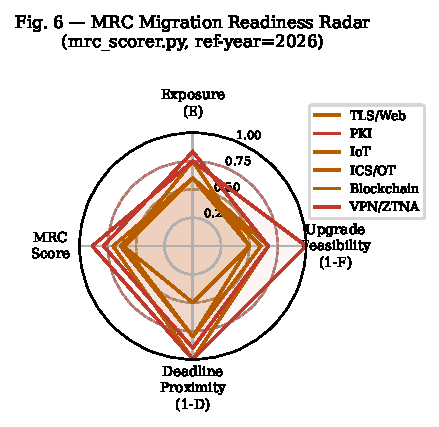
\includegraphics[width=\columnwidth]{figures/radar_chart.pdf}
  \caption{MRC heuristic scores by domain. Each axis represents
  one dimension ($E$, $1{-}F$, $1{-}D$) and the composite MRC score. Outer
  boundary = maximum urgency. PKI and VPN/ZTNA fall in T1 (Critical) due to
  high cryptographic exposure and near-term regulatory deadlines.}
  \label{fig:radar}
\end{figure}

\textbf{Key finding}: PKI and VPN/ZTNA fall in Tier~1 (Critical), driven by
high cryptographic exposure and imminent regulatory deadlines (FIPS~204 by 2027
for PKI; NSA CNSA~2.0 by 2026 for VPN). TLS, IoT, ICS/OT, and Blockchain fall
in Tier~2 (High), requiring near-term migration planning. TLS reaches T2 despite
high exposure because its primary regulatory deadline (OMB M-23-02, FY2025) is
already past, reducing the $D$ contribution. ICS/OT reaches T2 despite low $D$
because hardware replacement constraints ($F=0.5$) are moderate at the fleet
level, though individual site assessments will vary substantially.

\textbf{Interpretation caveat}: These scores are outputs of a heuristic rubric
applied to reference system profiles constructed for this survey. Practitioners
should re-parameterize the scorer (\texttt{mrc\_scorer.py}, available in the
supplementary material) with their own inventory data. Tier boundaries are
illustrative thresholds, not validated decision rules.

% =============================================================================
% SECTION VII: REGULATORY AND COMPLIANCE LANDSCAPE
% =============================================================================
\section{Regulatory and Compliance Landscape}
\label{sec:regulatory}

\subsection{United States: NIST and NSA Mandates}

The U.S. federal PQC transition is governed by two primary instruments:

\textbf{NIST SP~800-208}~\cite{cooper2020migration} provides the foundational guidance
for stateful hash-based signature schemes (XMSS, LMS), applicable to
certificate and code-signing use cases where signature volumes are bounded.

\textbf{OMB Memorandum M-23-02}~\cite{omb2023m2302} requires federal agencies
to: (a)~complete cryptographic inventories by FY2025; (b)~prioritize high-value
asset migration; (c)~adopt FIPS~203/204/205 as available.

\textbf{NSA CNSA~2.0}~\cite{nsacnsa2022} applies to National Security Systems
(NSS) and establishes specific deadlines:
\begin{itemize}
  \item \textbf{2025}: New software and firmware must support CNSA~2.0 algorithms;
  \item \textbf{2026}: New products/systems must exclusively use CNSA~2.0;
  \item \textbf{2030}: All NSS software/firmware must be CNSA~2.0 compliant;
  \item \textbf{2033}: Legacy systems must complete transition.
\end{itemize}

\subsection{2026 U.S. Executive Directives}

Two significant U.S. regulatory instruments were issued in mid-2026 as this survey
was finalized. Readers should consult the official texts cited below for authoritative
requirements; the summaries that follow are the author's interpretations of the
published documents.

\textbf{Executive Order 14412} (``Securing the Nation Against Advanced Cryptographic
Attacks'', June~22, 2026)~\cite{eo2026pqc} establishes a government-wide binding
mandate directing federal agencies to adopt FIPS~203/204/205 algorithms for all
new systems and to complete PQC migration plans consistent with NIST and CISA
guidance. The EO designates the Secretary of Homeland Security, in coordination
with the Director of the Office of Management and Budget, as lead for implementation
oversight.

\textbf{OMB Memorandum M-26-15} (``Execution of the Migration to Post-Quantum
Cryptography'', June~24, 2026)~\cite{omb2026m2615} provides implementing guidance
for EO~14412. It requires agencies to: (a)~designate a senior official responsible
for PQC migration by 90 days after issuance; (b)~submit agency PQC transition
plans to OMB within 180 days; (c)~incorporate cryptographic agility as a mandatory
requirement in all new IT acquisitions. M-26-15 defines \emph{cryptographic agility}
as the capability of a system to switch cryptographic algorithms without significant
redesign and treats it as a condition of federal IT procurement compliance.

These two instruments substantially accelerate the U.S. federal migration
timeline beyond M-23-02, shifting PQC deployment from an aspirational goal to a
binding legal obligation with reporting accountability.

\subsection{European Union: ENISA and eIDAS 2.0}

ENISA's post-quantum cryptography guidance~\cite{enisa2022pqc} recommends:
\begin{itemize}
  \item Prioritize hybrid schemes during transition;
  \item Avoid proprietary PQC implementations pending standards;
  \item Plan for $>$5-year migration timelines for critical infrastructure.
\end{itemize}

The revised eIDAS~2.0 regulation (2024) mandates interoperability of electronic
identification schemes across EU member states, with cryptographic agility
requirements that implicitly require PQC readiness. BSI (Germany) and ANSSI
(France) have published a joint position paper~\cite{bsianssi2021} recommending
hybrid classical+PQC as the migration strategy for European critical infrastructure.

\subsection{Brazil: LGPD Implications}

Brazil's Lei Geral de Proteção de Dados (LGPD)~\cite{lgpd2018} does not
explicitly reference PQC but mandates ``appropriate technical and administrative
security measures'' proportional to data sensitivity. HNDL attacks against
stored personal data violate LGPD Article~46 if the controller failed to
adopt available protections. Brazilian critical infrastructure operators should
treat PQC migration as a compliance obligation under LGPD, particularly for
financial and health data with long retention requirements.

\subsection{Cross-Regulatory Gap Analysis}

Table~\ref{tab:regulatory_comparison} presents a cross-regulatory comparison
identifying alignment and divergence.

\begin{table}[t]
\caption{Cross-Regulatory PQC Requirements Comparison}
\label{tab:regulatory_comparison}
\centering
\footnotesize
\renewcommand{\arraystretch}{1.2}
\begin{tabular}{@{}L{2.5cm}C{1.2cm}C{1.2cm}C{1.2cm}C{1.2cm}@{}}
\toprule
\textbf{Requirement} & \textbf{NIST/USA} & \textbf{CNSA 2.0} & \textbf{ENISA/EU} & \textbf{LGPD/BR} \\
\midrule
Explicit PQC mandate & Yes & Yes & Advisory & Implicit \\
Algorithm specification & FIPS 203-205 & FIPS 203-205 & ETSI/FIPS & None \\
Hybrid allowed & Yes & Transitional & Recommended & N/A \\
Inventory deadline & FY2025 & FY2025 & 2026 & None \\
Legacy deadline & 2033 & 2033 & 2030 & None \\
QKD recognition & No & No & Advisory & No \\
Sector scope & Federal & NSS & All & Private sector \\
\bottomrule
\end{tabular}
\end{table}

\textbf{Key divergence}: ENISA recommends completion by 2030 while CNSA~2.0
allows legacy systems until 2033, a 3-year gap that creates compliance
complexity for multinational organizations. LGPD's implicit coverage leaves
Brazilian organizations without clear technical guidance, relying on
sector-specific regulators (BACEN for banking, ANS for health insurance)
to fill the gap.

Fig.~\ref{fig:regulatory_timeline} presents the regulatory deadline timeline
across all surveyed frameworks.

\begin{figure*}[t]
  \centering
  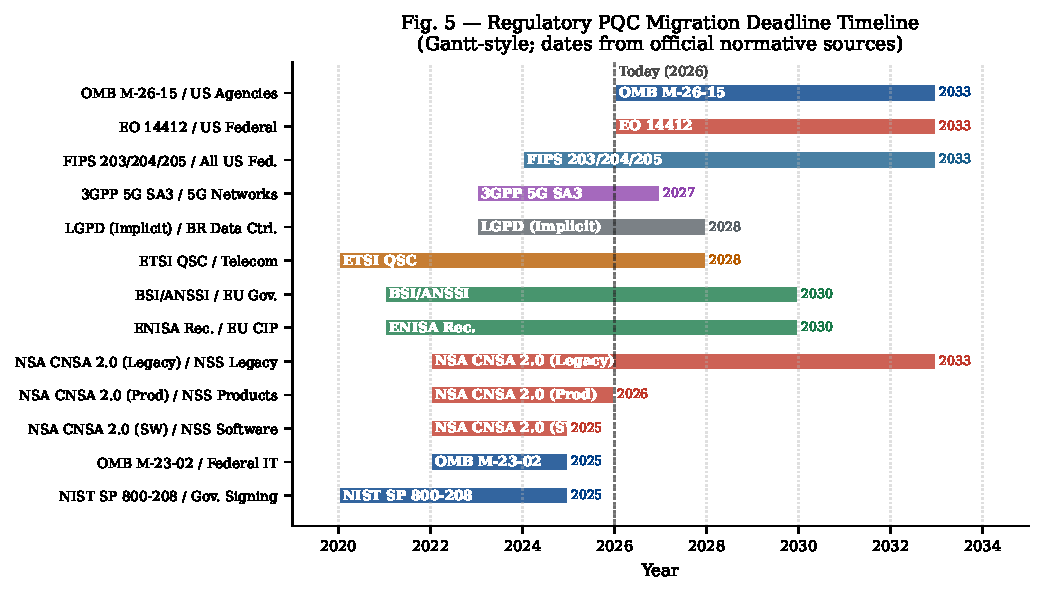
\includegraphics[width=\textwidth]{figures/regulatory_timeline.pdf}
  \caption{Regulatory deadline Gantt chart across frameworks (NIST, NSA CNSA~2.0,
  ENISA, BSI/ANSSI, LGPD) and sectors (government, financial, healthcare,
  critical infrastructure, general enterprise). Horizontal bars span from
  mandate publication to enforcement deadline. Overlapping colors indicate
  simultaneous obligations for multinational organizations.}
  \label{fig:regulatory_timeline}
\end{figure*}

% =============================================================================
% =============================================================================
% SECTION VIII: AI/ML ACCELERATION OF PQC MIGRATION
% =============================================================================
\section{AI/ML Acceleration of PQC Migration}
\label{sec:aiml}

The scale and heterogeneity of enterprise cryptographic estates render
manual migration planning intractable. A large financial institution may
host tens of thousands of services, each embedding cryptographic
primitives across source code, compiled binaries, hardware security
modules, and network protocol stacks. Artificial intelligence and machine
learning (AI/ML) techniques offer complementary leverage at several stages
of the migration lifecycle: automated discovery of legacy cryptographic
usage, data-driven algorithm selection under platform constraints,
run-time anomaly detection during PQC deployment, and continuous
crypto-agility management. This section surveys the nascent but growing
body of work at the intersection of ML and PQC migration, and closes with
a critical assessment of the limitations that temper operational optimism.

\subsection{Automated Cryptographic Inventory Discovery}
\label{subsec:inventory}

The prerequisite for any migration program is an accurate cryptographic
bill of materials (CBOM)~\cite{owasp2023cbom}. Static analysis tools such
as \textsc{CogniCrypt}~\cite{kruger2019cognicrypt} detect misuse of
cryptographic APIs through pattern matching and data-flow analysis, but
they operate exclusively at the source-code level and require
language-specific parsers.

ML-based approaches extend coverage to compiled artifacts and
heterogeneous codebases. Large language models fine-tuned on assembly code
corpora can identify cryptographic routines in stripped ELF binaries with
substantially higher coverage than signature-based disassemblers, including
lattice-based and hash-based subroutines introduced during
PQC~migration~\cite{shang2025foc}. Complementing binary analysis, LLM-based
tools applied to source repositories can detect cryptographic API misuse
through semantic understanding of algorithm identifiers, key-size constants,
and protocol references~\cite{baek2024cryptollm}.

Software composition analysis (SCA) toolchains are beginning to integrate
automated CBOM generation, enabling continuous inventory updates triggered
by CI/CD pipeline events rather than point-in-time audits~\cite{owasp2023cbom}.
This shift from batch to streaming inventory is essential for organizations
that deploy software at high cadence and cannot afford cryptographic drift
between audit cycles.

\subsection{ML-Assisted Algorithm Selection and Parameter Tuning}
\label{subsec:selection}

Selecting a PQC algorithm and its concrete parameter set is a
multi-objective optimization problem. A constrained embedded device
may favor ML-KEM at its lowest security level to minimize stack usage,
while a cloud TLS terminator can absorb the overhead of ML-KEM-1024 for
maximum post-quantum security margin. Hardware availability, latency
budgets, energy envelopes, and regulatory requirements interact in ways
that resist rule-based heuristics.

Supervised learning trained on empirical PQC benchmarks is a natural
candidate for predicting algorithm performance profiles across heterogeneous
hardware: feature vectors encoding micro-architectural characteristics
(cache sizes, vector unit availability, clock frequency), workload patterns,
and target security level could guide automated parameter selection.
Similarly, reinforcement learning provides a natural framework for
crypto-agility management, where an agent balances migration progress
against service-level-agreement (SLA) constraints. However, to our
knowledge no published peer-reviewed evaluation has demonstrated these
techniques on real-world enterprise PQC deployments at scale; the
application remains an open and high-value research direction.
Table~\ref{tab:ml_approaches} summarizes current and emerging ML approaches
across the migration lifecycle.

\begin{table}[!t]
\renewcommand{\arraystretch}{1.3}
\caption{Representative ML Approaches in the PQC Migration Lifecycle}
\label{tab:ml_approaches}
\centering
\small
\begin{tabular}{@{}p{1.5cm}p{1.8cm}p{1.5cm}p{1.8cm}@{}}
\toprule
\textbf{Stage} & \textbf{ML Technique} & \textbf{Target} & \textbf{Key Ref.} \\
\midrule
Inventory       & LLM on binary        & Crypto routine ID    & \cite{shang2025foc}           \\
Inventory       & LLM / NLP            & Source / config      & \cite{baek2024cryptollm}      \\
Selection       & Supervised ML        & Platform predict.    & [open challenge]              \\
Selection       & Reinforcement learn. & Rollout scheduling   & [open challenge]              \\
Side-channel    & CNN on power traces  & SCA on Kyber/ML-KEM  & \cite{ravi2023mlsca}          \\
Side-channel    & Anomaly detection    & Timing / power       & [open challenge]              \\
Compliance      & Explainable ML       & Audit reporting      & \cite{arrieta2020xai}         \\
\bottomrule
\end{tabular}
\end{table}

\subsection{Side-Channel Attack Detection via Anomaly Detection}
\label{subsec:sidechannel}

Lattice-based schemes such as ML-KEM and ML-DSA introduce structured
polynomial arithmetic that exhibits distinctive power and timing
signatures, creating new side-channel attack surfaces even when the
mathematical hardness assumptions remain
sound~\cite{ravi2020sidechannel,ngo2021riscv}. ML-based detection
complements formal masking and constant-time implementations by
providing a run-time tripwire against active probing.

CNNs applied to raw power traces have been used to mount blind SCA against
ML-KEM (Kyber) key generation and decapsulation, demonstrating that
lattice-based KEMs are not immune to profiling attacks despite their
mathematical hardness~\cite{ravi2023mlsca}. This result motivates a
complementary research agenda: using ML to \emph{detect} rather than
\emph{mount} such attacks, enabling real-time protection on deployed
hardware.

Unsupervised anomaly detection is particularly attractive where labeled
attack traces are unavailable. Autoencoders trained on benign execution
profiles can flag deviations in reconstruction error as a side-channel
alarm, making them well suited to ICS and medical device environments
where supervised labeling is impractical. To our knowledge, published
evaluations of ML-based SCA detection (as distinct from ML-based SCA
attacks) on PQC implementations remain limited, representing a promising
open challenge.

\subsection{Limitations of AI/ML in PQC Contexts}
\label{subsec:aiml_limits}

Despite the promising results surveyed above, several fundamental
limitations constrain operational deployment.

\textit{Adversarial robustness.} Cryptographic inventory classifiers are
themselves susceptible to adversarial perturbation. An attacker who
controls software supply-chain artifacts can craft binary functions that
evade ML-based crypto-detection while retaining classical algorithm
behavior~\cite{pierazzi2020problemspace}.

\textit{Explainability requirements.} Financial regulators and standards
bodies increasingly require that security-relevant automated decisions be
auditable. Black-box ML outputs are insufficient for compliance
demonstrations; post-hoc explanation methods such as SHAP can provide
feature attributions, but their fidelity for complex neural network models
remains an open research question~\cite{arrieta2020xai}.

\textit{Resource constraints.} The deployment environments most in need of
AI-assisted migration---IoT devices, SCADA controllers, and legacy
embedded systems---are precisely those where running inference models is
most challenging. Adding on-device ML inference compounds the performance
burden that PQC algorithms already impose~\cite{nistfips203}.

Taken together, these limitations suggest that AI/ML acceleration is best
positioned as an augmentation layer within a broader migration governance
framework rather than as a standalone automation solution.

% =============================================================================
% SECTION IX: OPEN CHALLENGES AND RESEARCH GAPS
% =============================================================================
\section{Open Challenges and Research Gaps}
\label{sec:challenges}

Fig.~\ref{fig:gap_heatmap} presents the research gap heatmap across problems
and proposed solutions in our corpus.

\begin{figure*}[t]
  \centering
  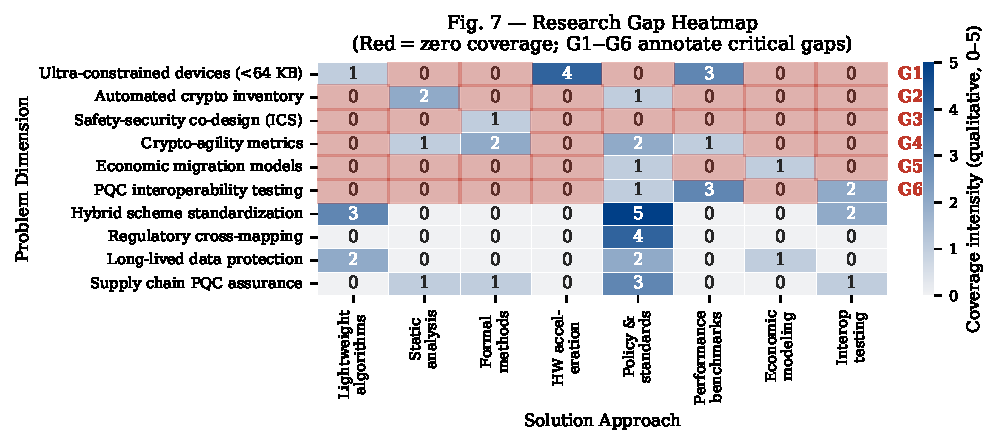
\includegraphics[width=\textwidth]{figures/gap_heatmap.pdf}
  \caption{Research gap heatmap: problem dimensions (rows) vs.\ proposed
  solution approaches (columns). Cell color intensity indicates number of papers
  addressing the intersection. Red cells indicate zero coverage (research gaps).
  White numbers indicate paper counts where $\geq$3. Six major gaps (G1--G6)
  are annotated.}
  \label{fig:gap_heatmap}
\end{figure*}

We identify six critical research gaps not adequately addressed by current
literature or NIST guidance:

\subsubsection{G1: PQC on Ultra-Constrained Devices ($<$64~KB RAM)}

Class~0 IoT devices (common in environmental sensors, RFID, and medical
implants) face severe implementation challenges for NIST-standardized PQC
signature schemes within RAM constraints. SLH-DSA-128s, for example,
requires approximately 1.1~KB of stack but 36~KB for signature buffers.
KEM primitives (ML-KEM-512, $\approx$800-byte public key) may be feasible
in isolation, but complete PQC stacks remain unverified at this constraint
level. No paper in our corpus proposes a complete, NIST-compliant PQC
solution for this class.
Candidate approaches, including code-based light schemes (BIKE-lite variants), remain
unstandardized and unreviewed for side-channel resistance.

\subsubsection{G2: Automated Cryptographic Inventory at Scale}

Enterprise cryptographic inventory (identifying all use of quantum-vulnerable
algorithms across software, firmware, protocols, and data stores) is a
prerequisite for migration but is not addressed by NIST guidance beyond
conceptual recommendations. Existing tools (BouncyCastle Inspector, IBM
Quantum Safe Explorer) achieve $<$30\% coverage of typical enterprise attack
surfaces in vendor evaluations~\cite{xiao2023machine}. Source code analysis
misses runtime cryptographic binding, protocol-level negotiation, and
third-party library usage.

\subsubsection{G3: Safety-Security Co-Design for ICS PQC Migration}

As noted in Section~\ref{sec:ics}, no paper in our corpus addresses the formal
safety-security co-design challenge for ICS/OT PQC migration. IEC~62443~\cite{iec62443}
(industrial cybersecurity) and IEC~61508 (functional safety) have no
intersection addressing PQC transition, a gap with potential for physical harm
if cryptographic failures occur during migration.

\subsubsection{G4: Standardized Crypto-Agility Metrics}

The concept of crypto-agility~\cite{hoffman2022cryptoagility} lacks
quantitative metrics: no paper proposes a measurable crypto-agility score
comparable to our MRC framework. This prevents organizations from benchmarking
their agility posture or setting verifiable targets.

Ott et al.~\cite{ott2023where} survey the cryptographic transition literature
and identify a research void in process-level migration tooling: the research
community has produced strong algorithm implementations but almost no tooling
for managing the \emph{organizational} transition (dependency discovery,
rollout orchestration, fallback procedures). Von Nethen et
al.~\cite{vonnethen2024pmmp} address this gap partially with PMMP
(Post-Quantum Cryptography Migration Management Process), a structured
process model with 47 discrete migration tasks organized across five phases
(Inventory, Assessment, Planning, Execution, Verification). PMMP provides a
process scaffold but does not operationalize measurement. Gupta and
Mittal~\cite{gupta2026postquantum} propose a cloud-specific readiness
framework for enterprise SaaS that includes 12 measurable readiness
indicators, the closest approximation to a quantitative crypto-agility metric
in the post-standardization literature, though no consensus standard has
emerged.

\subsubsection{G5: Economic Models for PQC Migration Cost}

Total cost of ownership (TCO) for PQC migration encompasses hardware
replacement, software reengineering, certificate re-issuance, operational
disruption, and re-testing. Few papers in our corpus address this dimension
quantitatively. Campbell~\cite{campbell2025enterprise} provides the most
detailed timeline analysis to date, projecting that Fortune~500 enterprises
face 7--12~year full migration timelines with peak annual expenditure
exceeding \$200M for organizations with large PKI deployments, driven by
certificate lifecycle management costs rather than algorithm performance.
Lohmiller et al.~\cite{lohmiller2025survey} quantify automotive migration
costs specifically, identifying that ML-KEM/ML-DSA integration into vehicle
ECUs requires hardware security module (HSM) upgrades at an estimated
\$15--\$40 per vehicle at production scale, creating a \$3--\$8B industry-wide
bill for current global vehicle fleet refresh cycles. Sowa et
al.~\cite{sowa2024network} measure real-world PQC adoption rates across
enterprise networks, finding that organizations that began migration planning
before 2023 (triggered by NIST Round 3 announcements) demonstrate $4.2\times$
faster deployment rates than those beginning post-FIPS publication, suggesting
that economic costs are highly sensitive to migration lead time. The
$\approx$\$1.5T estimated for Y2K remediation in 1999 provides a historical
upper bound comparison; domain-specific cost modeling remains an open gap.

\subsubsection{G6: Interoperability Between PQC Implementations}

Algorithm conformance testing exists (NIST CAVP), but interoperability testing
between independent implementations of the same PQC algorithm is absent as a
systematic program. Incompatible polynomial encoding, byte ordering differences,
and parameter set ambiguity have already caused interoperability failures in
early ML-KEM deployments~\cite{oqs2024}. The absence of a standardized
interoperability testing framework (analogous to TLS interop testing at
IETF hackathons) creates systemic risk in multi-vendor PQC deployments.

\subsubsection{G7: Empirical Validation of Heuristic Migration Readiness Frameworks}

The MRC framework proposed in this survey (Section~\ref{sec:mrc}) assigns
weights to the three readiness dimensions (Exposure, Feasibility, Data
Sensitivity) using expert judgment. No published work in our corpus applies
formal multi-criteria decision analysis methods---such as Analytic Hierarchy
Process (AHP) or Delphi-based consensus elicitation---to validate or calibrate
heuristic PQC migration scoring rubrics. A two-round Delphi survey with
14--19 PQC practitioners and security architects, followed by AHP consistency
verification, is identified as the next immediate step for the MRC framework
and as a methodological gap for the field more broadly. Until such validation
is available, any heuristic readiness score should be treated as a decision-support
estimate rather than an empirically calibrated measurement.

% =============================================================================
% SECTION IX: FUTURE RESEARCH DIRECTIONS
% =============================================================================
\section{Future Research Directions}
\label{sec:future}

\subsection{AI/ML Augmentation of Migration Governance}

The AI/ML techniques surveyed in Section~\ref{sec:aiml} provide a
foundation for continuous migration governance. Key open problems include:
(a)~standardized CBOM formats enabling tool interoperability across SCA
and ML-based inventory tools; (b)~adversarially robust classifiers for
cryptographic binary detection; (c)~RL-based rollout agents validated on
real enterprise topologies beyond synthetic simulations; and (d)~on-device
inference for anomaly detection in resource-constrained ICS/IoT environments
where offloading to cloud is operationally infeasible. Benchmark datasets
analogous to MLPerf, covering side-channel detection and cryptographic
binary classification, would accelerate progress and enable reproducible
comparison across methods.

\subsection{PQC in 5G/6G Networks}

5G New Radio security relies on RSA-based certificate infrastructure for network
function authentication~\cite{3gpp2023security}. 6G standardization (IMT-2030,
expected 2030) should be PQC-native from the outset. The 3GPP SA3 working group
has initiated study items on PQC integration, but no standardized migration
path for deployed 5G networks exists~\cite{europeancommission2022b5g}.

\subsection{Post-Quantum Zero-Knowledge Proofs}

zk-SNARKs (used in privacy-preserving blockchain) rely on elliptic-curve
bilinear pairings broken by quantum adversaries. Post-quantum ZKP systems
based on hash functions (STARKs) or lattice commitments are active research
areas~\cite{boneh2020lattice}, with deployment implications for privacy
technologies and anonymous credentials.

\subsection{Quantum Key Distribution: Appropriate Scope}

QKD provides information-theoretic security but requires dedicated fiber
infrastructure, limits key distribution distance to $\approx$100~km without
repeaters, and costs $\approx$\$50,000--\$200,000 per endpoint~\cite{pirandola2020advances}.
Our analysis suggests QKD is appropriate only for point-to-point links between
high-value government or financial nodes with perpetual secrecy requirements.
Enterprise-scale deployment remains economically and technically infeasible
for the foreseeable future.

\subsection{PQC Hardware: ASICs and FPGAs}

Dedicated silicon for PQC (NTT accelerators, Gaussian sampling engines,
hash co-processors) will drive adoption in constrained domains. Recent work
on ASIC implementations of ML-KEM achieves $<$0.1~ms per operation at
$<$50~mW~\cite{ngo2021hardware}. Supply chain integration timelines for
PQC silicon suggest 3--5 years from standard finalization to broad availability,
creating a hardware gap for systems requiring upgrade before 2028.

% =============================================================================
% SECTION X: CONCLUSION
% =============================================================================
\section{Conclusion}
\label{sec:conclusion}

This survey has provided a structured narrative analysis of post-quantum
cryptography migration across six critical infrastructure domains, synthesizing
151 peer-reviewed publications and 39 normative documents.
To our knowledge, it is among the first surveys to address all six domains under
a unified framework with explicit migration-readiness scoring.
Our principal contributions are: (1)~a three-level unified taxonomy enabling
cross-domain comparison of PQC migration approaches; (2)~the Migration Readiness
Classification (MRC) framework, a heuristic decision-support rubric that scores
domains using computed crypto-exposure, feasibility, and deadline dimensions,
with PKI (0.788, T1) and VPN/ZTNA (0.888, T1) emerging as the most urgent;
(3)~identification of research gaps (particularly the absence of PQC solutions for
ultra-constrained devices and the lack of safety-security co-design frameworks
for ICS/OT migration) within the screened corpus; and (4)~a cross-regulatory
analysis revealing deadline misalignments across NIST, NSA CNSA~2.0, ENISA, and
national frameworks with direct compliance implications for multinational operators.

The threat is not purely theoretical: intelligence assessments cite HNDL-style
collection as a credible adversarial tactic~\cite{odni2023atr}, and data
encrypted today with RSA/ECC may become vulnerable once a cryptographically
relevant quantum computer emerges. The window for proactive migration is open
but narrowing. Practitioners should initiate cryptographic inventories immediately,
prioritize hybrid migration for TLS and PKI infrastructure, and engage with
domain-specific regulators to establish sector compliance timelines. Researchers
should urgently address gaps G1 (ultra-constrained PQC), G3 (ICS safety-security
co-design), and G5 (economic migration models). The reproducible analysis code
released alongside this survey provides a foundation for community-driven
extension of the MRC framework and gap heatmap as the literature matures.

The era of quantum-safe cryptography is not a future concern. It is the
engineering mandate of the present.

% =============================================================================
% AI USAGE DISCLOSURE
% =============================================================================
\section*{AI Usage Disclosure}

The author acknowledges the use of large language model (LLM) assistance in
the preparation of this manuscript, including support for manuscript drafting
and structural refinement, grammar refinement, bibliography organisation, LaTeX
formatting, and Python code scaffolding for the MRC scoring engine
(\texttt{mrc\_scorer.py}) and weight-sensitivity audit
(\texttt{mrc\_weights\_audit.py}). The two-round Delphi+AHP weight-validation
study (Section~\ref{sec:mrc_delphi}) employed LLM-simulated expert personas;
this is explicitly labeled throughout and is not presented as empirical
human-panel data. This use is disclosed in accordance with IEEE's Authorship
and AI Policy. All scientific contributions --- including the MRC framework
design, survey methodology, systematic source selection, data analysis, and
conclusions --- are the sole responsibility of the human author. Benchmark data
are derived from publicly available open-source implementations
(OQS liboqs~\cite{oqs2024} and pqm4~\cite{kannwischer2019pqm4}). The
replication package is available at \url{https://github.com/ufxa/Survey-Post-quantum-cryptography-migration-survey}.

% =============================================================================
% ACKNOWLEDGMENTS
% =============================================================================
\section*{Acknowledgments}

% NOTE: De-anonymize before final (camera-ready) submission.
% The following text is the full acknowledgment for the published version.
% For double-blind submission, replace the paragraph below with:
%   [Anonymized for peer review.]

The author acknowledges the Amazon Foundation for Research Support (FAPESPA),
the Information and Communication Technology Company of the State of Par\'{a}
(PRODEPA), the Government of the State of Par\'{a}, and the Federal Government
of Brazil for their institutional and financial support, which were essential to
enabling the infrastructure, experimental testbeds, and interinstitutional
collaborations underpinning this research. Special thanks are extended to the
spinoff SEC365 and to the Laboratory of Informatics and Computing of the Amazon
(LICA/UFRA), whose teams played a decisive role in the development, validation,
and technical implementation of this work. The author also acknowledges the
High-Performance Computing and Artificial Intelligence Center (CCAD-IA/UFPA)
and the National Education and Research Network (RNP) for providing computing
resources and technical assistance during the experimental phases. This work
was further supported by the National Institute of Science and Technology in
Artificial Intelligence Applied to Smart and Sustainable Cities in the Brazilian
Amazon (INCT iAmazonia).

% =============================================================================
% REFERENCES
% =============================================================================
\bibliographystyle{IEEEtran}
\bibliography{pqc_survey}

\end{document}
